\chapter{Nevtralna geometrija}

    Geometrija brez aksioma o vzporednicah se imenuje \textbf{nevtralna geometrija}.

\section{Nevtralna geometrija}

    \begin{definicija}
        Naj bosta $p$ in $p'$ premici v nevtralni ravnini in $t$ prečnica, ki seka $p$ in $p'$ v točkah $B$ in $B'$. Izberimo točki $A\in p$ in $A'\in p'$ na nasprotnih bregovih premice $t$. Potem rečemo, da sta kota $\angle ABB'$ in $\angle A'B'B$ \textbf{izmenična kota}.
    \end{definicija}

    \begin{trditev}[I.27 -- izmenični notranji koti]
        Če premica $t$ seka premici $p$ in $q$ tako, da z njima oklepa par skladnih izmeničnih notranjih kotov, potem sta premici $p$ in $q$ vzporedni.
    \end{trditev}

        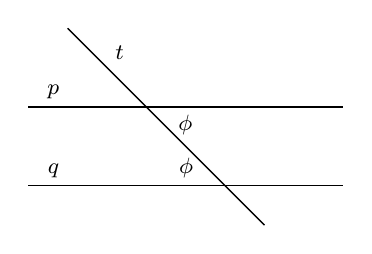
\begin{tikzpicture}
            % \clip (0,0) rectangle (14.000000,10.000000);
            {\footnotesize
            
            % Drawing line t'
            \draw [line width=0.016cm] (4.000000,2.000000) -- (1.500000,4.500000);%
            
            % Drawing line q'
            \draw [line width=0.016cm] (1.000000,2.500000) -- (5.000000,2.500000);%
            
            % Drawing line p'
            \draw [line width=0.016cm] (1.000000,3.500000) -- (5.000000,3.500000);%
            
            % Marking point p
            \draw (1.500000,3.500000) node [anchor=south east] { $p$ };%
            
            % Marking point q
            \draw (1.500000,2.500000) node [anchor=south east] { $q$ };%
            
            % Marking point t
            \draw (2.000000,4.000000) node [anchor=south west] { $t$ };%
            
            % Marking point \phi
            \draw (2.800000,3.500000) node [anchor=north west] { $\phi$ };%
            
            % Marking point \phi
            \draw (3.200000,2.500000) node [anchor=south east] { $\phi$ };%
            }
        \end{tikzpicture}

        \begin{dokaz}
            \\
            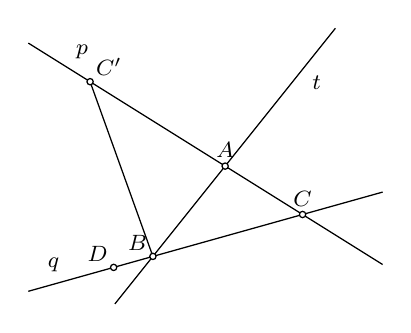
\begin{tikzpicture}
                % \clip (0,0) rectangle (14.000000,10.000000);
                {\footnotesize
                
                % Drawing line t'
                \draw [line width=0.016cm] (1.600000,1.000000) -- (2.057486,1.571858);%
                \draw [line width=0.016cm] (2.107462,1.634328) -- (2.975012,2.718765);%
                \draw [line width=0.016cm] (3.024988,2.781235) -- (4.400000,4.500000);%
                
                % Drawing line q'
                \draw [line width=0.016cm] (0.500000,1.160000) -- (1.545318,1.452689);%
                \draw [line width=0.016cm] (1.622355,1.474259) -- (2.043956,1.592308);%
                \draw [line width=0.016cm] (2.120993,1.613878) -- (3.944907,2.124574);%
                \draw [line width=0.016cm] (4.021944,2.146144) -- (5.000000,2.420000);%
                
                % Drawing line p'
                \draw [line width=0.016cm] (0.500000,4.312500) -- (1.250757,3.843277);%
                \draw [line width=0.016cm] (1.318597,3.800877) -- (2.966080,2.771200);%
                \draw [line width=0.016cm] (3.033920,2.728800) -- (3.949505,2.156559);%
                \draw [line width=0.016cm] (4.017345,2.114159) -- (5.000000,1.500000);%
                
                % Marking point p
                \draw (1.000000,4.000000) node [anchor=south west] { $p$ };%
                
                % Marking point q
                \draw (1.000000,1.300000) node [anchor=south east] { $q$ };%
                
                % Marking point t
                \draw (4.000000,4.000000) node [anchor=north west] { $t$ };%
                
                % Marking point A by circle
                \draw [line width=0.016cm] (3.000000,2.750000) circle (0.040000);%
                \draw (3.000000,2.750000) node [anchor=south] { $A$ };%
                
                % Marking point B by circle
                \draw [line width=0.016cm] (2.082474,1.603093) circle (0.040000);%
                \draw (2.112474,1.573093) node [anchor=south east] { $B$ };%
                
                % Marking point C by circle
                \draw [line width=0.016cm] (3.983425,2.135359) circle (0.040000);%
                \draw (3.983425,2.135359) node [anchor=south] { $C$ };%
                
                % Marking point D by circle
                \draw [line width=0.016cm] (1.583836,1.463474) circle (0.040000);%
                \draw (1.613836,1.433474) node [anchor=south east] { $D$ };%
                
                % Marking point C' by circle
                \draw [line width=0.016cm] (1.284677,3.822077) circle (0.040000);%
                \draw (1.254677,3.792077) node [anchor=south west] { $C'$ };%
                
                % Drawing segment B C'
                \draw [line width=0.016cm] (2.068941,1.640734) -- (1.298210,3.784436);%
                }
            \end{tikzpicture}
            \\ Denimo, da se $p$ in $q$ sekata. Izberimo $C'\in p$ tako, da je $C\ast A\ast C'$ in $AC'\cong BC$. Iz SKS sledi: $\angle ABC \cong \angle BAC'$ in $\angle BAC\cong \angle ABC'$. Potem je, zaradi $\angle DBA\cong \angle BAC\cong \angle ABC'$, točka $C'$ na poltraku $\overrightarrow{BD}$: $p$ in $q$ se sekata v dveh točkah, torej sta ista premica. To pa je protislovje. 
        \end{dokaz}

    \begin{posledica} ~
        \begin{enumerate}[label=\arabic*$)$]
            \item Če za $p$ in $q$ obstaja skupna pravokotnica, potem sta $p$ in $q$ vzporedni.
            \item Za vsako premico $p$ in točko $A\notin p$ obstaja vzporednica k $p$ skozi $A$.
        \end{enumerate}
    \end{posledica}

        \begin{dokaz}
            \begin{enumerate}[label=\arabic*$)$]
                \item Sledi iz trditve in skladnosti pravih kotov.
                \item Naj bo $t$ pravokotnica na $p$ skozi $A$ in $q$ pravokotnica na $t$ skozi $A$. Po točki $1)$ sta $p$ in $q$ vzporedni.
            \end{enumerate}
            \begin{tikzpicture}
                % \clip (0,0) rectangle (14.000000,10.000000);
                {\footnotesize
                
                % Drawing line p'
                \draw [line width=0.016cm] (1.000000,2.000000) -- (5.000000,2.000000);%
                
                % Drawing line q'
                \draw [line width=0.016cm] (1.000000,3.500000) -- (2.460000,3.500000);%
                \draw [line width=0.016cm] (2.540000,3.500000) -- (5.000000,3.500000);%
                
                % Drawing line t'
                \draw [line width=0.016cm] (2.500000,1.500000) -- (2.500000,3.460000);%
                \draw [line width=0.016cm] (2.500000,3.540000) -- (2.500000,4.500000);%
                
                % Marking point p
                \draw (4.000000,2.000000) node [anchor=south east] { $p$ };%
                
                % Marking point q
                \draw (3.944670,3.500000) node [anchor=south east] { $q$ };%
                
                % Marking point t
                \draw (2.500000,3.954070) node [anchor=south east] { $t$ };%
                
                % Marking point A by circle
                \draw [line width=0.016cm] (2.500000,3.500000) circle (0.040000);%
                \draw (2.530000,3.470000) node [anchor=south east] { $A$ };%
                }
            \end{tikzpicture}
        \end{dokaz}

    \begin{opomba}
        Evklid prvič uporabi E.5 (aksiom o vzporednicah) v dokazu obrata prejšnje trditve I.27.
    \end{opomba}

    Naslednja trditev v nevtralni geometriji ne velja.
    \begin{trditev}[I.29]
        Če sta $p\parallel q$ in $t$ seka $p$ in $q$, potem sta izmenična notranja kota skladna.
    \end{trditev}

    \begin{posledica}
        Naj bo $p$ premica in $A$ točka. Potem obstaja natanko ena pravokotnica na $p$ skozi točko $A$.
    \end{posledica}

        \begin{dokaz}
            \begin{enumerate}[label=\arabic*$)$]
                \item $A\in p$: Potem to sledi iz skladnosti pravih kotov.
                \\ \begin{tikzpicture}
                    % \clip (0,0) rectangle (14.000000,10.000000);
                    {\footnotesize
                    
                    % Drawing line p'
                    \draw [line width=0.016cm] (1.000000,1.900000) -- (2.866459,2.273292);%
                    \draw [line width=0.016cm] (2.944906,2.288981) -- (5.000000,2.700000);%
                    
                    % Drawing line t'
                    \draw [line width=0.016cm] (3.061910,1.500000) -- (2.913527,2.241913);%
                    \draw [line width=0.016cm] (2.897838,2.320360) -- (2.661910,3.500000);%
                    
                    % Marking point p
                    \draw (4.000000,2.500000) node [anchor=south east] { $p$ };%
                    
                    % Marking point A by circle
                    \draw [line width=0.016cm] (2.905683,2.281137) circle (0.040000);%
                    \draw (2.935683,2.311137) node [anchor=north east] { $A$ };%
                    }
                \end{tikzpicture}
                \item $A\notin p$: Če sta pravokotnici na $p$ različni, bi morali biti vzporedni, imata pa skupno točko $A$.
                \\ \begin{tikzpicture}
                    % \clip (0,0) rectangle (14.000000,10.000000);
                    {\footnotesize
                    
                    % Drawing line B A
                    \draw [line width=0.016cm] (2.824904,1.500000) -- (2.996511,3.460152);%
                    \draw [line width=0.016cm] (3.003489,3.539848) -- (3.043774,4.000000);%
                    
                    % Drawing line p'
                    \draw [line width=0.016cm] (1.000000,1.916667) -- (5.000000,2.583333);%
                    
                    % Drawing line t'
                    \draw [line width=0.016cm] (3.333333,1.500000) -- (3.006576,3.460544);%
                    \draw [line width=0.016cm] (2.993424,3.539456) -- (2.916667,4.000000);%
                    
                    % Marking point p
                    \draw (4.500000,2.500000) node [anchor=south east] { $p$ };%
                    
                    % Marking point A by circle
                    \draw [line width=0.016cm] (3.000000,3.500000) circle (0.040000);%
                    \draw (3.000000,3.500000) node [anchor=west] { $A$ };%
                    }
                \end{tikzpicture}
            \end{enumerate}
        \end{dokaz}

    \begin{trditev}[I.16 - Izrek o zunanjem kotu]
        Zunanji kot trikotnika je večji od kateregakoli nasprotnega notranjega kota.
    \end{trditev}

        \begin{dokaz}
            \\ \dashuline{$\angle C < \angle CBD$}
            \\ Recimo, da to ne velja. Potem obstajata dve možnosti.
            \begin{enumerate}[label=\arabic*$)$]
                \item $\angle C\cong \angle CBD$: Tedaj bi premici $\overleftrightarrow{AC}$ in $\overleftrightarrow{AB}$ oklepali skladna izmenična notranja kota s premico $\overleftrightarrow{BC}$ in bi bili vzporedni $\overleftrightarrow{AC}\parallel\overleftrightarrow{AB}$. PROTISLOVJE 
                \item $\angle C > \angle CBD$: Potem obstaja točka $E\in\angle ACB$ taka, da je $\angle ECB\cong\angle DBC$. Kot prej sta $\overleftrightarrow{CE}\parallel\overleftrightarrow{AB}$. Po izreku o prečnici $\overleftrightarrow{CE}$ seka $AB$. PROTISLOVJE
            \end{enumerate}
            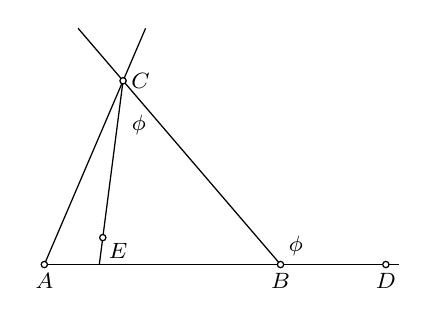
\begin{tikzpicture}
                % \clip (0,0) rectangle (14.000000,10.000000);
                {\footnotesize
                
                % Drawing segment A H
                \draw [line width=0.016cm] (1.540000,1.500000) -- (4.460000,1.500000);%
                \draw [line width=0.016cm] (4.540000,1.500000) -- (5.797306,1.500000);%
                \draw [line width=0.016cm] (5.877306,1.500000) -- (6.000000,1.500000);%
                
                % Drawing segment G C
                \draw [line width=0.016cm] (2.198294,1.500000) -- (2.237380,1.802280);%
                \draw [line width=0.016cm] (2.247638,1.881619) -- (2.494871,3.793664);%
                
                % Drawing segment A J
                \draw [line width=0.016cm] (1.515757,1.536766) -- (2.484243,3.796568);%
                \draw [line width=0.016cm] (2.515757,3.870099) -- (2.785714,4.500000);%
                
                % Drawing segment B I
                \draw [line width=0.016cm] (4.473968,1.530370) -- (2.526032,3.802963);%
                \draw [line width=0.016cm] (2.473968,3.863704) -- (1.928571,4.500000);%
                
                % Marking point A by circle
                \draw [line width=0.016cm] (1.500000,1.500000) circle (0.040000);%
                \draw (1.500000,1.500000) node [anchor=north] { $A$ };%
                
                % Marking point B by circle
                \draw [line width=0.016cm] (4.500000,1.500000) circle (0.040000);%
                \draw (4.500000,1.500000) node [anchor=north] { $B$ };%
                
                % Marking point C by circle
                \draw [line width=0.016cm] (2.500000,3.833333) circle (0.040000);%
                \draw (2.500000,3.833333) node [anchor=west] { $C$ };%
                
                % Marking point D by circle
                \draw [line width=0.016cm] (5.837306,1.500000) circle (0.040000);%
                \draw (5.837306,1.500000) node [anchor=north] { $D$ };%
                
                % Marking point E by circle
                \draw [line width=0.016cm] (2.242509,1.841950) circle (0.040000);%
                \draw (2.212509,1.871950) node [anchor=north west] { $E$ };%
                
                % Marking point \phi
                \draw (2.700000,3.500000) node [anchor=north] { $\phi$ };%
                
                % Marking point \phi
                \draw (4.500000,1.500000) node [anchor=south west] { $\phi$ };%
                }
            \end{tikzpicture}
        \end{dokaz}

    \begin{posledica}[I.17]
        Vsota mer poljubnih dveh kotov trikotnika je manjša kot $\pi$.
    \end{posledica}

        \begin{dokaz}
            \\
            \begin{tikzpicture}
                % \clip (0,0) rectangle (14.000000,10.000000);
                {\footnotesize
                
                % Drawing segment C I
                \draw [line width=0.016cm] (1.540000,1.500000) -- (4.960000,1.500000);%
                \draw [line width=0.016cm] (5.040000,1.500000) -- (6.000000,1.500000);%
                
                % Drawing segment A C
                \draw [line width=0.016cm] (2.976000,3.468000) -- (1.524000,1.532000);%
                
                % Drawing segment B A
                \draw [line width=0.016cm] (4.971716,1.528284) -- (3.028284,3.471716);%
                
                % Marking point A by circle
                \draw [line width=0.016cm] (3.000000,3.500000) circle (0.040000);%
                \draw (3.000000,3.500000) node [anchor=south] { $A$ };%
                
                % Marking point B by circle
                \draw [line width=0.016cm] (5.000000,1.500000) circle (0.040000);%
                \draw (5.000000,1.500000) node [anchor=north] { $B$ };%
                
                % Marking point C by circle
                \draw [line width=0.016cm] (1.500000,1.500000) circle (0.040000);%
                \draw (1.500000,1.500000) node [anchor=north] { $C$ };%
                
                % Marking point \alpha
                \draw (3.000000,3.300000) node [anchor=north] { $\alpha$ };%
                
                % Marking point \beta
                \draw (4.500000,1.500000) node [anchor=south] { $\beta$ };%
                
                % Marking point \pi-\beta
                \draw (5.300000,1.500000) node [anchor=south] { $\pi-\beta$ };%
                }
            \end{tikzpicture}               
            \\ Po trditvi I.16 je: $\angle A < zunanji~ kot~ pri~ B$; $|\angle A| < |zunanji~ kot~ pri~ B|$; $\alpha < \pi - \beta$ ~$\Rightarrow \alpha+\beta<\pi$.
        \end{dokaz}

    \begin{trditev}[I.26 - SKK]
        Naj za trikotnika $\triangle ABC$ in $\triangle DEF$ velja: $AB\cong DE$, $\angle B\cong \angle E$ in $\angle C\cong \angle F$. \\
        Potem sta trikotnika $\triangle ABC$ in $\triangle DEF$ skladna.
    \end{trditev}

        \begin{dokaz}
            \\
            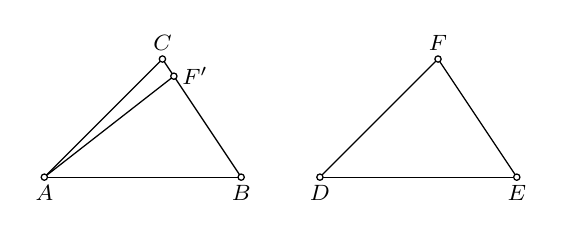
\begin{tikzpicture}
                % \clip (0,0) rectangle (14.000000,10.000000);
                {\footnotesize
                
                % Drawing segment A B
                \draw [line width=0.016cm] (1.540000,1.500000) -- (3.960000,1.500000);%
                
                % Drawing segment A C
                \draw [line width=0.016cm] (1.528284,1.528284) -- (2.971716,2.971716);%
                
                % Drawing segment B C
                \draw [line width=0.016cm] (3.977812,1.533282) -- (3.167365,2.748953);%
                \draw [line width=0.016cm] (3.122989,2.815517) -- (3.022188,2.966718);%
                
                % Drawing segment D E
                \draw [line width=0.016cm] (5.040000,1.500000) -- (7.460000,1.500000);%
                
                % Drawing segment D F
                \draw [line width=0.016cm] (5.028284,1.528284) -- (6.471716,2.971716);%
                
                % Drawing segment E F
                \draw [line width=0.016cm] (7.477812,1.533282) -- (6.522188,2.966718);%
                
                % Drawing segment A F'
                \draw [line width=0.016cm] (1.531549,1.524589) -- (3.113627,2.757646);%
                
                % Marking point A by circle
                \draw [line width=0.016cm] (1.500000,1.500000) circle (0.040000);%
                \draw (1.500000,1.500000) node [anchor=north] { $A$ };%
                
                % Marking point B by circle
                \draw [line width=0.016cm] (4.000000,1.500000) circle (0.040000);%
                \draw (4.000000,1.500000) node [anchor=north] { $B$ };%
                
                % Marking point C by circle
                \draw [line width=0.016cm] (3.000000,3.000000) circle (0.040000);%
                \draw (3.000000,3.000000) node [anchor=south] { $C$ };%
                
                % Marking point D by circle
                \draw [line width=0.016cm] (5.000000,1.500000) circle (0.040000);%
                \draw (5.000000,1.500000) node [anchor=north] { $D$ };%
                
                % Marking point E by circle
                \draw [line width=0.016cm] (7.500000,1.500000) circle (0.040000);%
                \draw (7.500000,1.500000) node [anchor=north] { $E$ };%
                
                % Marking point F by circle
                \draw [line width=0.016cm] (6.500000,3.000000) circle (0.040000);%
                \draw (6.500000,3.000000) node [anchor=south] { $F$ };%
                
                % Marking point F' by circle
                \draw [line width=0.016cm] (3.145177,2.782235) circle (0.040000);%
                \draw (3.145177,2.782235) node [anchor=west] { $F'$ };%
                }
            \end{tikzpicture}                
            \\ Če je $BC\cong EF$, sta trikotnika skladna po kriteriju SKS.
            Denimo, da velja $BC\ncong EF$, naj bo $EF<BC$. Potem obstaja točka $F'$, da je $BF'\cong EF$ in $B\ast F'\ast C$. Tako po SKS sledi $\triangle ABF'\cong\triangle DEF$ in $\angle C\cong \angle F\cong \angle AF'B$. To pa je v protislovju s tem, da je kot $\angle AF'B$ zunanji za trikotnik $\triangle ACF'$ in skladen z nasprotnim notranjim kotom $\angle C$.
        \end{dokaz}

    \begin{trditev}[skladnost pravokotnih trikotnikov]
        Če imata pravokotna trikotnika skladni hipotenuzi in po eno kateto, potem sta skladna.
    \end{trditev}

        \begin{dokaz}
            \\
            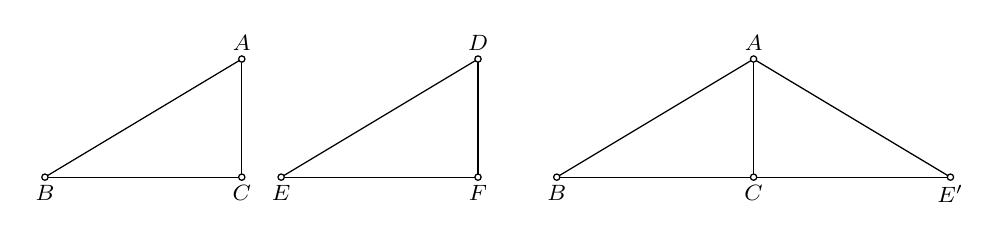
\begin{tikzpicture}
                % \clip (0,0) rectangle (14.000000,10.000000);
                {\footnotesize
                
                % Drawing segment A B
                \draw [line width=0.016cm] (3.965700,2.979420) -- (1.534300,1.520580);%
                
                % Drawing segment A C
                \draw [line width=0.016cm] (4.000000,2.960000) -- (4.000000,1.540000);%
                
                % Drawing segment B C
                \draw [line width=0.016cm] (1.540000,1.500000) -- (3.960000,1.500000);%
                
                % Drawing segment D E
                \draw [line width=0.016cm] (6.965700,2.979420) -- (4.534300,1.520580);%
                
                % Drawing segment D F
                \draw [line width=0.016cm] (7.000000,2.960000) -- (7.000000,1.540000);%
                
                % Drawing segment E F
                \draw [line width=0.016cm] (4.540000,1.500000) -- (6.960000,1.500000);%
                
                % Marking point A by circle
                \draw [line width=0.016cm] (4.000000,3.000000) circle (0.040000);%
                \draw (4.000000,3.000000) node [anchor=south] { $A$ };%
                
                % Marking point B by circle
                \draw [line width=0.016cm] (1.500000,1.500000) circle (0.040000);%
                \draw (1.500000,1.500000) node [anchor=north] { $B$ };%
                
                % Marking point C by circle
                \draw [line width=0.016cm] (4.000000,1.500000) circle (0.040000);%
                \draw (4.000000,1.500000) node [anchor=north] { $C$ };%
                
                % Marking point D by circle
                \draw [line width=0.016cm] (7.000000,3.000000) circle (0.040000);%
                \draw (7.000000,3.000000) node [anchor=south] { $D$ };%
                
                % Marking point E by circle
                \draw [line width=0.016cm] (4.500000,1.500000) circle (0.040000);%
                \draw (4.500000,1.500000) node [anchor=north] { $E$ };%
                
                % Marking point F by circle
                \draw [line width=0.016cm] (7.000000,1.500000) circle (0.040000);%
                \draw (7.000000,1.500000) node [anchor=north] { $F$ };%
                
                % Drawing segment A B
                \draw [line width=0.016cm] (10.465700,2.979420) -- (8.034300,1.520580);%
                
                % Drawing segment A C
                \draw [line width=0.016cm] (10.500000,2.960000) -- (10.500000,1.540000);%
                
                % Drawing segment B C
                \draw [line width=0.016cm] (8.040000,1.500000) -- (10.460000,1.500000);%
                
                % Drawing segment A E'
                \draw [line width=0.016cm] (10.534300,2.979420) -- (12.965700,1.520580);%
                
                % Drawing segment C E'
                \draw [line width=0.016cm] (10.540000,1.500000) -- (12.960000,1.500000);%
                
                % Marking point A by circle
                \draw [line width=0.016cm] (10.500000,3.000000) circle (0.040000);%
                \draw (10.500000,3.000000) node [anchor=south] { $A$ };%
                
                % Marking point B by circle
                \draw [line width=0.016cm] (8.000000,1.500000) circle (0.040000);%
                \draw (8.000000,1.500000) node [anchor=north] { $B$ };%
                
                % Marking point C by circle
                \draw [line width=0.016cm] (10.500000,1.500000) circle (0.040000);%
                \draw (10.500000,1.500000) node [anchor=north] { $C$ };%
                
                % Marking point E' by circle
                \draw [line width=0.016cm] (13.000000,1.500000) circle (0.040000);%
                \draw (13.000000,1.500000) node [anchor=north] { $E'$ };%
                }
            \end{tikzpicture}                
            \\ Naj bo točka $E'$ na $\overleftrightarrow{BC}$ taka, da je: $B\ast C\ast E'$ in $CE'\cong EF$.
            Iz SKS sledi: $\triangle ACE'\cong\triangle DFE$. V trikotniku $\triangle ABE'$ je $AB\cong AE'$, torej je enakokrak in sta kota ob osnovnici $BE'$ skladna ($\angle B\cong\angle E'\cong \angle E$). Po kriteriju SKK sledi: $\triangle ACB\cong\triangle DFE$.
        \end{dokaz}

    \begin{definicija}
        \textbf{Simetrala kota} $\angle AOB$ v nevtralni ravnini je poltrak $\overrightarrow{OT}$, ki zadošča pogojema: $T$ je v notranjosti kota $\angle AOB$ in $\angle AOT\cong\angle BOT$.
    \end{definicija}

    \begin{definicija}
        \textbf{Simetrala daljice} $AB$ v nevtralni ravnini je premica $s_{AB}$, za katero velja: simetrala $s_{AB}$ seka daljico $AB$ v točki $T$, za katero je $TA\cong TB$ in $s_{AB}\perp\overleftrightarrow{AB}$.
    \end{definicija}

    \begin{trditev}
        Vsak kot ima simetralo in vsaka stranica ima simetralo.
    \end{trditev}

        \begin{dokaz}
            \\ (simetrala kota): Izberimo točko $B'$ na poltraku $\overrightarrow{OB}$, da bo $OA\cong OB'$. Ozančimo s $T$ pravokotno projekcijo točke $O$ na premico $\overleftrightarrow{AB'}$. Trikotnik $\triangle OAB'$ je enakokrak, od koder sledi, da sta $\angle OAB'\cong\angle OB'A$ ostra kota. Če bi točka $T$ ležala izven daljice $AB'$, bi bil v trikotnik $\triangle OB'T$ oziroma $\triangle OAT$ zunanji kot pri $B'$ oziroma $A$ manjši kot pravi kot pri $T$. Od tod sledi, da leži točka $T$ v notranjosti daljice $AB'$. Za trikotnika $\triangle AOT$ in $\triangle B'OT$ velja $\angle OTA\cong \angle OTB'$ in $\angle OAT\cong \angle OB'T$. Torej imata skladna dva para kotov in skupno stranico $OT$. Zato  sta po kriteriju KKS skladna. Od tod pa sledi $\angle AOT\cong\angle B'OT$.
            \\
            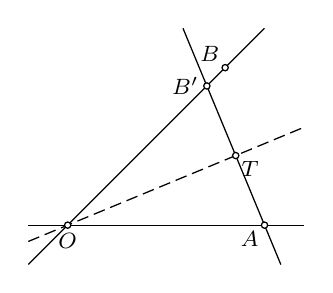
\begin{tikzpicture}
                % \clip (0,0) rectangle (14.000000,10.000000);
                {\footnotesize
                
                % Drawing line s
                \draw [line width=0.016cm] (1.000000,1.292893) -- (1.138582,1.350296);%
                \draw [line width=0.016cm] (1.207873,1.378997) -- (1.346455,1.436400);%
                \draw [line width=0.016cm] (1.415746,1.465101) -- (1.463045,1.484693);%
                \draw [line width=0.016cm] (1.536955,1.515307) -- (1.554328,1.522503);%
                \draw [line width=0.016cm] (1.623619,1.551205) -- (1.762201,1.608607);%
                \draw [line width=0.016cm] (1.831492,1.637308) -- (1.970074,1.694711);%
                \draw [line width=0.016cm] (2.039364,1.723412) -- (2.177946,1.780815);%
                \draw [line width=0.016cm] (2.247237,1.809516) -- (2.385819,1.866918);%
                \draw [line width=0.016cm] (2.455110,1.895620) -- (2.593692,1.953022);%
                \draw [line width=0.016cm] (2.662983,1.981723) -- (2.801565,2.039126);%
                \draw [line width=0.016cm] (2.870856,2.067827) -- (3.009438,2.125230);%
                \draw [line width=0.016cm] (3.078729,2.153931) -- (3.217311,2.211333);%
                \draw [line width=0.016cm] (3.286602,2.240035) -- (3.425184,2.297437);%
                \draw [line width=0.016cm] (3.494475,2.326138) -- (3.596928,2.368576);%
                \draw [line width=0.016cm] (3.702348,2.412242) -- (3.840930,2.469645);%
                \draw [line width=0.016cm] (3.910221,2.498346) -- (4.048802,2.555749);%
                \draw [line width=0.016cm] (4.118093,2.584450) -- (4.256675,2.641852);%
                \draw [line width=0.016cm] (4.325966,2.670554) -- (4.464548,2.727956);%
                
                % Drawing line t
                \draw [line width=0.016cm] (4.207107,1.000000) -- (4.015307,1.463045);%
                \draw [line width=0.016cm] (3.984693,1.536955) -- (3.649191,2.346928);%
                \draw [line width=0.016cm] (3.618576,2.420839) -- (3.283074,3.230812);%
                \draw [line width=0.016cm] (3.252460,3.304722) -- (2.964466,4.000000);%
                
                % Drawing line a
                \draw [line width=0.016cm] (1.000000,1.500000) -- (1.460000,1.500000);%
                \draw [line width=0.016cm] (1.540000,1.500000) -- (3.960000,1.500000);%
                \draw [line width=0.016cm] (4.040000,1.500000) -- (4.500000,1.500000);%
                
                % Drawing line b
                \draw [line width=0.016cm] (1.000000,1.000000) -- (1.471716,1.471716);%
                \draw [line width=0.016cm] (1.528284,1.528284) -- (3.239483,3.239483);%
                \draw [line width=0.016cm] (3.296051,3.296051) -- (3.471716,3.471716);%
                \draw [line width=0.016cm] (3.528284,3.528284) -- (4.000000,4.000000);%
                
                % Marking point O by circle
                \draw [line width=0.016cm] (1.500000,1.500000) circle (0.040000);%
                \draw (1.500000,1.500000) node [anchor=north] { $O$ };%
                
                % Marking point A by circle
                \draw [line width=0.016cm] (4.000000,1.500000) circle (0.040000);%
                \draw (4.030000,1.530000) node [anchor=north east] { $A$ };%
                
                % Marking point B by circle
                \draw [line width=0.016cm] (3.500000,3.500000) circle (0.040000);%
                \draw (3.530000,3.470000) node [anchor=south east] { $B$ };%
                
                % Marking point B' by circle
                \draw [line width=0.016cm] (3.267767,3.267767) circle (0.040000);%
                \draw (3.267767,3.267767) node [anchor=east] { $B'$ };%
                
                % Marking point T by circle
                \draw [line width=0.016cm] (3.633883,2.383883) circle (0.040000);%
                \draw (3.603883,2.413883) node [anchor=north west] { $T$ };%
                }
            \end{tikzpicture}
            \\ (simetrala stranice): Izberemo enakokrak trikotnik $\triangle ABC$, ki ima $AB$ za osnovnico. Označimo s $T$ pravokotno projekcijo točke $C$ na $AB$. Po definiciji, seka premica $\overleftrightarrow{CT}$ daljico $AB$ pravokotno. Za trikotnika $\triangle ACT$ in $\triangle BCT$ velja $\angle TAC\cong \angle TBC$, $\angle ATC\cong\angle BTC$, imata pa trikotnika tudi skupno stranico $CT$. Po kriteriju KKS je zato $\triangle ACT \cong \triangle BCT$, od koder sledi $AT\cong BT$.
            \\
            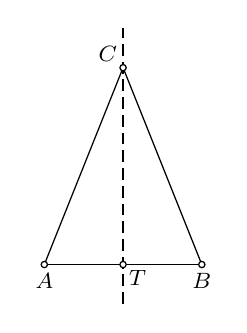
\begin{tikzpicture}
                % \clip (0,0) rectangle (14.000000,10.000000);
                {\footnotesize
                
                % Drawing segment A B
                \draw [line width=0.016cm] (2.040000,1.500000) -- (2.960000,1.500000);%
                \draw [line width=0.016cm] (3.040000,1.500000) -- (3.960000,1.500000);%
                
                % Drawing segment B C
                \draw [line width=0.016cm] (3.985144,1.537139) -- (3.014856,3.962861);%
                
                % Drawing segment A C
                \draw [line width=0.016cm] (2.014856,1.537139) -- (2.985144,3.962861);%
                
                % Marking point A by circle
                \draw [line width=0.016cm] (2.000000,1.500000) circle (0.040000);%
                \draw (2.000000,1.500000) node [anchor=north] { $A$ };%
                
                % Marking point B by circle
                \draw [line width=0.016cm] (4.000000,1.500000) circle (0.040000);%
                \draw (4.000000,1.500000) node [anchor=north] { $B$ };%
                
                % Marking point C by circle
                \draw [line width=0.016cm] (3.000000,4.000000) circle (0.040000);%
                \draw (3.030000,3.970000) node [anchor=south east] { $C$ };%
                
                % Marking point T by circle
                \draw [line width=0.016cm] (3.000000,1.500000) circle (0.040000);%
                \draw (2.970000,1.530000) node [anchor=north west] { $T$ };%
                
                % Drawing line s
                \draw [line width=0.016cm] (3.000000,1.000000) -- (3.000000,1.150000);%
                \draw [line width=0.016cm] (3.000000,1.225000) -- (3.000000,1.375000);%
                \draw [line width=0.016cm] (3.000000,1.450000) -- (3.000000,1.460000);%
                \draw [line width=0.016cm] (3.000000,1.540000) -- (3.000000,1.600000);%
                \draw [line width=0.016cm] (3.000000,1.675000) -- (3.000000,1.825000);%
                \draw [line width=0.016cm] (3.000000,1.900000) -- (3.000000,2.050000);%
                \draw [line width=0.016cm] (3.000000,2.125000) -- (3.000000,2.275000);%
                \draw [line width=0.016cm] (3.000000,2.350000) -- (3.000000,2.500000);%
                \draw [line width=0.016cm] (3.000000,2.575000) -- (3.000000,2.725000);%
                \draw [line width=0.016cm] (3.000000,2.800000) -- (3.000000,2.950000);%
                \draw [line width=0.016cm] (3.000000,3.025000) -- (3.000000,3.175000);%
                \draw [line width=0.016cm] (3.000000,3.250000) -- (3.000000,3.400000);%
                \draw [line width=0.016cm] (3.000000,3.475000) -- (3.000000,3.625000);%
                \draw [line width=0.016cm] (3.000000,3.700000) -- (3.000000,3.850000);%
                \draw [line width=0.016cm] (3.000000,3.925000) -- (3.000000,3.960000);%
                \draw [line width=0.016cm] (3.000000,4.040000) -- (3.000000,4.075000);%
                \draw [line width=0.016cm] (3.000000,4.150000) -- (3.000000,4.300000);%
                \draw [line width=0.016cm] (3.000000,4.375000) -- (3.000000,4.500000);%
                }
            \end{tikzpicture}                
        \end{dokaz}


    \begin{trditev}[I.18, I.19]
        V trikotniku leži večji kot nasproti večje/daljše stranice in obratno, večja stranica leži nasproti večjega kota.
    \end{trditev}

        \begin{dokaz}
            \\
            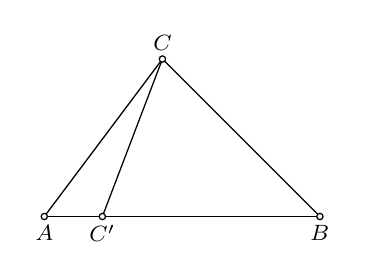
\begin{tikzpicture}
                % \clip (0,0) rectangle (14.000000,10.000000);
                {\footnotesize
                
                % Drawing segment A B
                \draw [line width=0.016cm] (1.540000,1.500000) -- (2.197236,1.500000);%
                \draw [line width=0.016cm] (2.277236,1.500000) -- (4.960000,1.500000);%
                
                % Drawing segment A C
                \draw [line width=0.016cm] (1.524000,1.532000) -- (2.976000,3.468000);%
                
                % Drawing segment B C
                \draw [line width=0.016cm] (4.971716,1.528284) -- (3.028284,3.471716);%
                
                % Drawing segment C C'
                \draw [line width=0.016cm] (2.985746,3.462626) -- (2.251489,1.537374);%
                
                % Marking point A by circle
                \draw [line width=0.016cm] (1.500000,1.500000) circle (0.040000);%
                \draw (1.500000,1.500000) node [anchor=north] { $A$ };%
                
                % Marking point B by circle
                \draw [line width=0.016cm] (5.000000,1.500000) circle (0.040000);%
                \draw (5.000000,1.500000) node [anchor=north] { $B$ };%
                
                % Marking point C by circle
                \draw [line width=0.016cm] (3.000000,3.500000) circle (0.040000);%
                \draw (3.000000,3.500000) node [anchor=south] { $C$ };%
                
                % Marking point C' by circle
                \draw [line width=0.016cm] (2.237236,1.500000) circle (0.040000);%
                \draw (2.237236,1.500000) node [anchor=north] { $C'$ };%
                }
            \end{tikzpicture}                
            \\ ($\Rightarrow$):
            \\ Naj bo $AB>BC$. Trdimo: $\angle C>\angle A$. Potem obstaja točka $C'$ taka, da je $A\ast C'\ast B$ in $BC\cong BC'$. $\Rightarrow$ Trikotnik $\triangle BCC'$ je enakokrak z vrhom v $B$. Torej velja $\angle CC'B\cong\angle C'CB$. Od tod sledi: $\uline{\angle A<} \angle CC'B\cong\angle C'CB\uline{<\angle C}$.
            \\ ($\Leftarrow$):
            \\ Denimo, da je $\angle C >\angle A$. Trdimo: $AB>BC$. Če to ni res, potem je $AB\leq BC$:\begin{enumerate}
                \item $AB<BC$: Po prejšnji trditvi sledi $\angle C <\angle A$ --- PROTISLOVJE 
                \item $AB\cong BC$: Zaradi enakokrakosti trikotnika je $\angle A\cong\angle C$ --- PROTISLOVJE
            \end{enumerate}
        \end{dokaz}

    \begin{posledica}[I.20 -- trikotniška neenakost]
        Če točke $A,B,C$ niso kolinearne, potem je $|AC|<|AB|+|BC|$.
    \end{posledica}

        \begin{dokaz}
            \\
            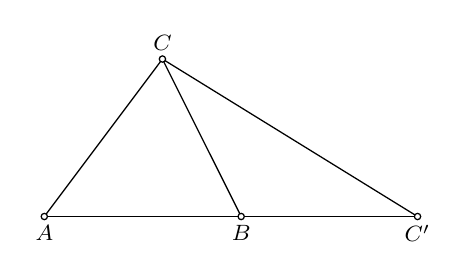
\begin{tikzpicture}
                % \clip (0,0) rectangle (14.000000,10.000000);
                {\footnotesize
                
                % Drawing segment A C'
                \draw [line width=0.016cm] (1.540000,1.500000) -- (3.960000,1.500000);%
                \draw [line width=0.016cm] (4.040000,1.500000) -- (6.200000,1.500000);%
                
                % Drawing segment A C
                \draw [line width=0.016cm] (1.524000,1.532000) -- (2.976000,3.468000);%
                
                % Drawing segment B C
                \draw [line width=0.016cm] (3.982111,1.535777) -- (3.017889,3.464223);%
                
                % Drawing segment C C'
                \draw [line width=0.016cm] (3.034037,3.478989) -- (6.205963,1.521011);%
                
                % Marking point A by circle
                \draw [line width=0.016cm] (1.500000,1.500000) circle (0.040000);%
                \draw (1.500000,1.500000) node [anchor=north] { $A$ };%
                
                % Marking point B by circle
                \draw [line width=0.016cm] (4.000000,1.500000) circle (0.040000);%
                \draw (4.000000,1.500000) node [anchor=north] { $B$ };%
                
                % Marking point C by circle
                \draw [line width=0.016cm] (3.000000,3.500000) circle (0.040000);%
                \draw (3.000000,3.500000) node [anchor=south] { $C$ };%
                
                % Marking point C' by circle
                \draw [line width=0.016cm] (6.240000,1.500000) circle (0.040000);%
                \draw (6.240000,1.500000) node [anchor=north] { $C'$ };%
                }
            \end{tikzpicture}                
            \\ Na premici $\overleftrightarrow{AB}$ izberemo točko $C'$, da je $A\ast B\ast C'$ in $BC\cong BC'$.
            Točka $B$ je v notranjosti kota $\angle ACC'$, od koder sledi, da je $\angle BCC' < \angle ACC'$.
            Trikotnik $\triangle C'CB$ je enakokrak, od koder sledi $\angle AC'C \cong \angle BCC'$.
            V trikotniku $\triangle AC'C$ je torej $\angle AC'C < \angle ACC'$ in zato je $AC<AC'$.
            Ker je $AC'\cong AB+BC$, je $AC<AB+BC$.
        \end{dokaz}

    \begin{trditev}[I.24, I.25]
        Naj za trikotnika $\triangle ABC$ in $\triangle A'B'C'$ velja: $AB\cong A'B'$ in $AC\cong A'C'$.
        Potem je: $\angle A > \angle A' \Leftrightarrow BC > B'C'$.
    \end{trditev}

        \begin{dokaz}
            \\ ($\Rightarrow$):
            \\ Recimo, da je $\angle A > \angle A'$. Izberimo točko $C''$ v notranjosti kota $\angle A$, tako, da bo veljalo $\angle BAC'' \cong \angle B'A'C'$ in $AC''\cong A'C'$. Po predpostavki naloge je tudi $AB\cong A'B'$, zato sta po kriteriju SKS trikotnika $\triangle ABC''$ in $\triangle A'B'C'$ skladna. Poleg tega iz $AC''\cong AC$ sledi, da je trikotnika $\triangle AC''C$ enakokrak in je zato $\angle AC''C\cong \angle ACC''$.
            Ker je točka $C''$ v notranjosti kota $\angle BAC$, poltrak $\overrightarrow{AC''}$ seka daljico $BC$ v točki, ki jo bomo označili z $D$. Glede na lego točke $D$ ločimo tri možnosti: \begin{enumerate}
                \item \uline{$A\ast D\ast C''$:} Ker je $A$ v notranjosti kota $\angle BC''C$, je $\angle BC''C>\angle AC''C$ in tudi $\angle BC''C > \angle ACC''$. Podobno iz dejstva, da je $B$ v notranjosti kota $\angle ACC''$ sledi, da je $\angle ACC'' > \angle BCC''$. V trikotniku $\triangle BC''C$ je torej $\angle BC''C>\angle BCC''$, zato je po izreku s predavanj $BC>BC''$ in posledično $BC>B'C'$. 
                \\ 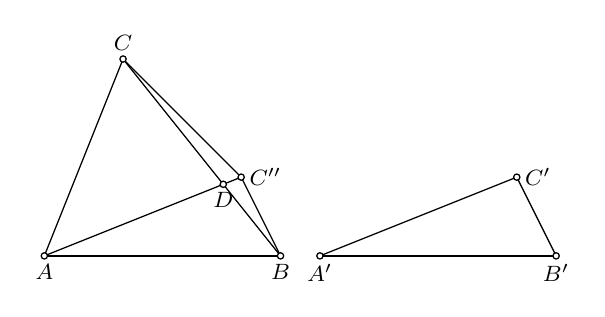
\begin{tikzpicture}
                    % \clip (0,0) rectangle (14.000000,10.000000);
                    {\footnotesize
                    
                    % Drawing segment A B
                    \draw [line width=0.016cm] (1.540000,1.500000) -- (4.460000,1.500000);%
                    
                    % Drawing segment A C
                    \draw [line width=0.016cm] (1.514856,1.537139) -- (2.485144,3.962861);%
                    
                    % Drawing segment A C''
                    \draw [line width=0.016cm] (1.537139,1.514856) -- (3.735588,2.394235);%
                    \draw [line width=0.016cm] (3.809866,2.423947) -- (3.962861,2.485144);%
                    
                    % Drawing segment C B
                    \draw [line width=0.016cm] (2.524988,3.968765) -- (3.747739,2.440326);%
                    \draw [line width=0.016cm] (3.797715,2.377856) -- (4.475012,1.531235);%
                    
                    % Drawing segment B C''
                    \draw [line width=0.016cm] (4.482111,1.535777) -- (4.017889,2.464223);%
                    
                    % Drawing segment C C''
                    \draw [line width=0.016cm] (2.528284,3.971716) -- (3.971716,2.528284);%
                    
                    % Drawing segment A' B'
                    \draw [line width=0.016cm] (5.040000,1.500000) -- (7.960000,1.500000);%
                    
                    % Drawing segment A' C'
                    \draw [line width=0.016cm] (5.037139,1.514856) -- (7.462861,2.485144);%
                    
                    % Drawing segment B' C'
                    \draw [line width=0.016cm] (7.982111,1.535777) -- (7.517889,2.464223);%
                    
                    % Marking point A by circle
                    \draw [line width=0.016cm] (1.500000,1.500000) circle (0.040000);%
                    \draw (1.500000,1.500000) node [anchor=north] { $A$ };%
                    
                    % Marking point B by circle
                    \draw [line width=0.016cm] (4.500000,1.500000) circle (0.040000);%
                    \draw (4.500000,1.500000) node [anchor=north] { $B$ };%
                    
                    % Marking point A' by circle
                    \draw [line width=0.016cm] (5.000000,1.500000) circle (0.040000);%
                    \draw (5.000000,1.500000) node [anchor=north] { $A'$ };%
                    
                    % Marking point B' by circle
                    \draw [line width=0.016cm] (8.000000,1.500000) circle (0.040000);%
                    \draw (8.000000,1.500000) node [anchor=north] { $B'$ };%
                    
                    % Marking point C by circle
                    \draw [line width=0.016cm] (2.500000,4.000000) circle (0.040000);%
                    \draw (2.500000,4.000000) node [anchor=south] { $C$ };%
                    
                    % Marking point C' by circle
                    \draw [line width=0.016cm] (7.500000,2.500000) circle (0.040000);%
                    \draw (7.500000,2.500000) node [anchor=west] { $C'$ };%
                    
                    % Marking point C'' by circle
                    \draw [line width=0.016cm] (4.000000,2.500000) circle (0.040000);%
                    \draw (4.000000,2.500000) node [anchor=west] { $C''$ };%
                    
                    % Marking point D by circle
                    \draw [line width=0.016cm] (3.772727,2.409091) circle (0.040000);%
                    \draw (3.772727,2.409091) node [anchor=north] { $D$ };%
                    }
                \end{tikzpicture}                    
                \item \uline{$D=C''$:} V tem primeru je $BC''+C''C\cong BC$ in zato iz $BC''\cong B'C'$ sledi $BC>B'C'$.
                \item \uline{$A\ast C''\ast D$:} Tokrat je točka $D$ v notranjosti kota $\angle BC''C$, zato je  $\angle BC''C>\angle DC''C$. Kot $\angle DC''C$ je zunanji kot v trikotniku $\triangle AC''C$, od koder sledi $\angle DC''C > \angle ACC''$. Ker je trikotnik $\triangle AC''C$ enakokrak, je posledično $\angle ACC''\cong \angle AC''C$: Kot  $\angle AC''C$ pa je zunanji kot v trikotniku $\triangle C''DC$, od koder dobimo še $\angle AC''C > \angle C''CB$. Tako smo prišli do neenakosti $\angle BC''C > \angle DC''C > \angle ACC'' \cong \angle AC''C > \angle C''CB$. V trikotniku $\triangle BC''C$ torej velja $BC>BC''\cong B'C'$, kar smo želeli pokazati.
                \\ 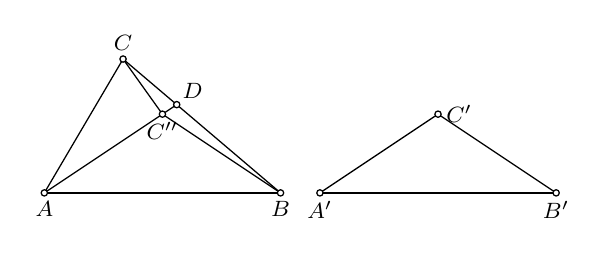
\begin{tikzpicture}
                    % \clip (0,0) rectangle (14.000000,10.000000);
                    {\footnotesize
                    
                    % Drawing segment A B
                    \draw [line width=0.016cm] (1.540000,1.500000) -- (4.460000,1.500000);%
                    
                    % Drawing segment A C
                    \draw [line width=0.016cm] (1.520281,1.534477) -- (2.479719,3.165523);%
                    
                    % Drawing segment A D
                    \draw [line width=0.016cm] (1.533282,1.522188) -- (2.966718,2.477812);%
                    \draw [line width=0.016cm] (3.033282,2.522188) -- (3.148037,2.598691);%
                    
                    % Drawing segment C B
                    \draw [line width=0.016cm] (2.530478,3.174094) -- (3.150841,2.646785);%
                    \draw [line width=0.016cm] (3.211796,2.594973) -- (4.469522,1.525906);%
                    
                    % Drawing segment B C''
                    \draw [line width=0.016cm] (4.466718,1.522188) -- (3.033282,2.477812);%
                    
                    % Drawing segment C C''
                    \draw [line width=0.016cm] (2.523250,3.167451) -- (2.976750,2.532549);%
                    
                    % Drawing segment A' B'
                    \draw [line width=0.016cm] (5.040000,1.500000) -- (7.960000,1.500000);%
                    
                    % Drawing segment A' C'
                    \draw [line width=0.016cm] (5.033282,1.522188) -- (6.466718,2.477812);%
                    
                    % Drawing segment B' C'
                    \draw [line width=0.016cm] (7.966718,1.522188) -- (6.533282,2.477812);%
                    
                    % Marking point A by circle
                    \draw [line width=0.016cm] (1.500000,1.500000) circle (0.040000);%
                    \draw (1.500000,1.500000) node [anchor=north] { $A$ };%
                    
                    % Marking point B by circle
                    \draw [line width=0.016cm] (4.500000,1.500000) circle (0.040000);%
                    \draw (4.500000,1.500000) node [anchor=north] { $B$ };%
                    
                    % Marking point A' by circle
                    \draw [line width=0.016cm] (5.000000,1.500000) circle (0.040000);%
                    \draw (5.000000,1.500000) node [anchor=north] { $A'$ };%
                    
                    % Marking point B' by circle
                    \draw [line width=0.016cm] (8.000000,1.500000) circle (0.040000);%
                    \draw (8.000000,1.500000) node [anchor=north] { $B'$ };%
                    
                    % Marking point C by circle
                    \draw [line width=0.016cm] (2.500000,3.200000) circle (0.040000);%
                    \draw (2.500000,3.200000) node [anchor=south] { $C$ };%
                    
                    % Marking point C' by circle
                    \draw [line width=0.016cm] (6.500000,2.500000) circle (0.040000);%
                    \draw (6.500000,2.500000) node [anchor=west] { $C'$ };%
                    
                    % Marking point C'' by circle
                    \draw [line width=0.016cm] (3.000000,2.500000) circle (0.040000);%
                    \draw (3.000000,2.500000) node [anchor=north] { $C''$ };%
                    
                    % Marking point D by circle
                    \draw [line width=0.016cm] (3.181319,2.620879) circle (0.040000);%
                    \draw (3.151319,2.590879) node [anchor=south west] { $D$ };%
                    }
                \end{tikzpicture}                    
            \end{enumerate}
            ($\Leftarrow$):
            \\ Recimo sedaj, da je $BC>B'C'$. Po izreku o trihotomiji imamo tri možnosti: \begin{enumerate}
                \item $\angle BAC > \angle B'A'C'$
                \item $\angle BAC \cong \angle B'A'C'$
                \item $\angle BAC < \angle B'A'C'$
            \end{enumerate}
            Če bi bilo $\angle BAC \cong \angle B'A'C'$, bi bila po kriteriju SKS trikotnika $\triangle ABC$ in $\triangle A'B'C'$ skladna. Posledično bi bilo $BC\cong B'C'$, kar pa je v protislovju s predpostavko $BC>B'C'$.
            \\ Če bi bilo $\angle BAC < \angle B'A'C'$, pa bi po pravkar dokazanem od tod sledilo $BC<B'C'$, kar je spet v protislovju s predpostavko.
            \\ Tako nam ostane samo še možnosti $\angle BAC > \angle B'A'C'$, ki smo jo želeli dokazati.
        \end{dokaz}

    \begin{izrek}[Merjenje kotov]
        Obstaja natanko ena funkcija, ki vsakemu kotu $\angle A$ priredi mero $|\angle A|$ (v radianih) in ima naslednje lastnosti:
        \begin{enumerate}
            \item $|\angle A| \in (0, \pi)$.
            \item $|\angle A|=\frac{\pi}{2}$ natanko tedaj, ko je $\angle A$ pravi kot.
            \item $|\angle A| = |\angle B|$ natanko tedaj, ko je $\angle A\cong \angle B$.
            \item Če $\overrightarrow{AC}$ leži v notranjosti $\angle DAB$, potem je $|\angle DAB|=|\angle DAC| + |\angle CAB|$.
            \item $|\angle A| < |\angle B|$ natanko tedaj, ko velja $\angle A < \angle B$.
            \item Za vsak $x\in(0,\pi)$ obstaja kot $\angle A$ z $|\angle A|=x$.
            \item Vsota mer suplementarnih kotov je enaka $\pi$.
        \end{enumerate}
    \end{izrek}

    \begin{izrek}[Merjenje daljic]
        Naj bo dana daljica $OI$, ki jo imenujemo \textbf{enotska daljica}. Potem obstaja natanko ena funkcija, ki vsaki daljici $AB$ priredi dolžino $|AB|$ in ima naslednje lastnosti:
        \begin{enumerate}
            \item $|AB|>0$ in $|OI|=1$.
            \item $|AB|=|CD|$ natanko tedaj, ko velja $AB\cong CD$.
            \item $A\ast B\ast C$ natanko tedaj, ko velja $|AC|=|AB|+|BC|$.
            \item $|AB|<|CD|$ natanko tedaj, ko velja $AB<CD$.
            \item Za vsako pozitivno realno število $x$ obstaja daljica $AB$ z $|AB|=x$.
        \end{enumerate}
    \end{izrek}

    \begin{opomba}
        V hiperbolični geometriji pa obstaja tudi naravna enota za dolžino. To je povezano s skladnostnim kriterijem KKK.
    \end{opomba}

    \begin{izrek}[Legandre-Saccheri]
        Vsota mer notranjih kotov v poljubnem trikotniku je manjša ali enaka $\pi$.
    \end{izrek}

        \begin{dokaz}
            \\ Recimo, da obstaja trikotnik $\triangle ABC$, da velja: $\alpha+\beta+\gamma=\pi+\epsilon; \epsilon>0$. Ideja je, da poiščemo trikotnik z enako vsoto kotov in enim kotom manjšim od $\epsilon$. (protislovje --  vsota preostalih dveh kotov večja/enaka $\pi$)
            \\ Naj bo točka $D$ razpolovišče $BC$ in točka $E$ na poltraku $\overrightarrow{AD}$ taka, da je $A\ast D\ast E$ in $AD\cong DE$.
            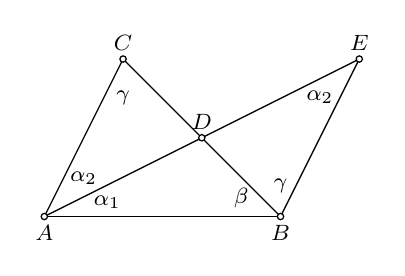
\begin{tikzpicture}
                % \clip (0,0) rectangle (14.000000,10.000000);
                {\footnotesize
                
                % Drawing segment A C
                \draw [line width=0.016cm] (1.517889,1.535777) -- (2.482111,3.464223);%
                
                % Drawing segment A B
                \draw [line width=0.016cm] (1.540000,1.500000) -- (4.460000,1.500000);%
                
                % Drawing segment B C
                \draw [line width=0.016cm] (4.471716,1.528284) -- (3.528284,2.471716);%
                \draw [line width=0.016cm] (3.471716,2.528284) -- (2.528284,3.471716);%
                
                % Drawing segment B E
                \draw [line width=0.016cm] (4.517889,1.535777) -- (5.482111,3.464223);%
                
                % Drawing segment A E
                \draw [line width=0.016cm] (1.535777,1.517889) -- (3.464223,2.482111);%
                \draw [line width=0.016cm] (3.535777,2.517889) -- (5.464223,3.482111);%
                
                % Marking point A by circle
                \draw [line width=0.016cm] (1.500000,1.500000) circle (0.040000);%
                \draw (1.500000,1.500000) node [anchor=north] { $A$ };%
                
                % Marking point B by circle
                \draw [line width=0.016cm] (4.500000,1.500000) circle (0.040000);%
                \draw (4.500000,1.500000) node [anchor=north] { $B$ };%
                
                % Marking point C by circle
                \draw [line width=0.016cm] (2.500000,3.500000) circle (0.040000);%
                \draw (2.500000,3.500000) node [anchor=south] { $C$ };%
                
                % Marking point E by circle
                \draw [line width=0.016cm] (5.500000,3.500000) circle (0.040000);%
                \draw (5.500000,3.500000) node [anchor=south] { $E$ };%
                
                % Marking point D by circle
                \draw [line width=0.016cm] (3.500000,2.500000) circle (0.040000);%
                \draw (3.500000,2.500000) node [anchor=south] { $D$ };%
                
                % Marking point \gamma
                \draw (2.500000,3.200000) node [anchor=north] { $\gamma$ };%
                
                % Marking point \gamma
                \draw (4.500000,1.700000) node [anchor=south] { $\gamma$ };%
                
                % Marking point \beta
                \draw (4.000000,1.500000) node [anchor=south] { $\beta$ };%
                
                % Marking point \alpha_1
                \draw (2.300000,1.500000) node [anchor=south] { $\alpha_1$ };%
                
                % Marking point \alpha_2
                \draw (2.000000,1.800000) node [anchor=south] { $\alpha_2$ };%
                
                % Marking point \alpha_2
                \draw (5.000000,3.200000) node [anchor=north] { $\alpha_2$ };%
                }
            \end{tikzpicture}                
            \\ \dashuline{Vsota kotov v $\triangle ABE$ je $\pi+\epsilon$.}
            \\ Po kriteriju SKS velja: $\triangle ADC\cong \triangle EDB$. Vsota kotov trikotnika $\triangle ABE$ je: $\alpha_1+\beta+\gamma+\alpha_2=\alpha+\beta+\gamma=\pi+\epsilon$. V trikotniku $\triangle ABE$ sta notranja kota $\alpha_1$ in $\alpha_2$ z vsoto $\alpha$, torej je vsaj eden manjši/enak $\frac{\alpha}{2}$. Če ta postopek ponavljamo, po nekaj korakih dobimo trikotnik z enako vsoto kotov in enim kotom manjšim od $\epsilon$, kar pa nas pripelje v protislovje.
        \end{dokaz}

    \begin{opomba}
        V sferični geometriji to ni res: vsota notranjih kotov poljubnega sferičnega trikotnika je večja od $\pi$.
    \end{opomba}

    \begin{posledica}
        Vsota mer dveh notranjih kotov trikotnika je manjša/enaka meri nasprotnega zunanjega kota.
    \end{posledica}

    \begin{definicija}
        \textbf{Defekt} trikotnika $\triangle ABC$ je $\delta(\triangle ABC)=\pi-(\alpha+\beta+\gamma)$.
    \end{definicija}

    \begin{posledica}
        $\delta(\triangle ABC)\geq 0$
    \end{posledica}

    \begin{trditev}
        Naj velja $A\ast D\ast B$. Potem je $\delta(\triangle ABC)=\delta(\triangle ADC)+\delta(\triangle DBC)$.
    \end{trditev}

        \begin{dokaz}
            \\
            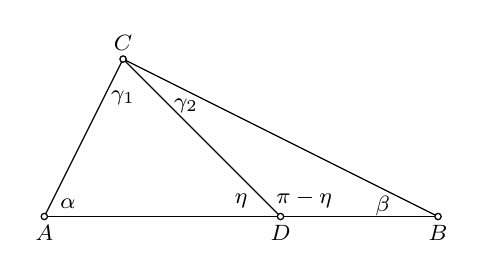
\begin{tikzpicture}
                % \clip (0,0) rectangle (14.000000,10.000000);
                {\footnotesize
                
                % Drawing segment A C
                \draw [line width=0.016cm] (1.517889,1.535777) -- (2.482111,3.464223);%
                
                % Drawing segment A B
                \draw [line width=0.016cm] (1.540000,1.500000) -- (4.460000,1.500000);%
                \draw [line width=0.016cm] (4.540000,1.500000) -- (6.460000,1.500000);%
                
                % Drawing segment B C
                \draw [line width=0.016cm] (6.464223,1.517889) -- (2.535777,3.482111);%
                
                % Drawing segment C D
                \draw [line width=0.016cm] (2.528284,3.471716) -- (4.471716,1.528284);%
                
                % Marking point A by circle
                \draw [line width=0.016cm] (1.500000,1.500000) circle (0.040000);%
                \draw (1.500000,1.500000) node [anchor=north] { $A$ };%
                
                % Marking point B by circle
                \draw [line width=0.016cm] (6.500000,1.500000) circle (0.040000);%
                \draw (6.500000,1.500000) node [anchor=north] { $B$ };%
                
                % Marking point C by circle
                \draw [line width=0.016cm] (2.500000,3.500000) circle (0.040000);%
                \draw (2.500000,3.500000) node [anchor=south] { $C$ };%
                
                % Marking point D by circle
                \draw [line width=0.016cm] (4.500000,1.500000) circle (0.040000);%
                \draw (4.500000,1.500000) node [anchor=north] { $D$ };%
                
                % Marking point \gamma_1
                \draw (2.500000,3.200000) node [anchor=north] { $\gamma_1$ };%
                
                % Marking point \gamma_2
                \draw (3.300000,3.100000) node [anchor=north] { $\gamma_2$ };%
                
                % Marking point \beta
                \draw (5.800000,1.400000) node [anchor=south] { $\beta$ };%
                
                % Marking point \alpha
                \draw (1.800000,1.500000) node [anchor=south] { $\alpha$ };%
                
                % Marking point \etha
                \draw (4.000000,1.500000) node [anchor=south] { $\eta$ };%
                
                % Marking point \pi-\etha
                \draw (4.800000,1.500000) node [anchor=south] { $\pi-\eta$ };%
                }
            \end{tikzpicture}                
            \\ $\delta(\triangle ADC)=\pi-(\alpha+\eta +\gamma_1)=\pi-\alpha-\eta-\gamma_1$
            \\ $\delta(\triangle DBC)=\pi-(\pi-\eta+\beta +\gamma_2)=\eta-\beta-\gamma_2$
            \\ $\delta(\triangle ADC)+\delta(\triangle DBC)=\pi-\alpha-\beta-\gamma_1-\gamma_2= \pi-(\alpha+\beta+\gamma)=\delta(\triangle ABC)$
        \end{dokaz}

    \begin{opomba}
        Defekt se obnaša podobno kot ploščina -- v primeru, da je $\delta>0$, ga res lahko uporabimo za merjenje ploščine.
    \end{opomba}

    \begin{posledica}
        Naj bo $A\ast D\ast B$. Potem je $\delta(\triangle ABC)=0 \Leftrightarrow \delta(\triangle ADC)=0$ in $\delta(\triangle DBC)=0$.
    \end{posledica}

    \begin{definicija}
        \textbf{Pravokotnik} je štirikotnik, v katerem so vsi štirje koti pravi.
    \end{definicija}

    \begin{izrek}[obstoj pravokotnikov]
        ~
        \begin{enumerate}
            \item Če obstaja trikotnik z $\delta=0$, potem obstaja pravokotnik.
            \item Če obstaja pravokotnik, imajo vsi trikotniki $\delta=0$.
        \end{enumerate}
    \end{izrek}

        \begin{dokaz}
            \begin{enumerate}
                \item Naj bo $\delta(\triangle ABC)=0$. 
                \\ 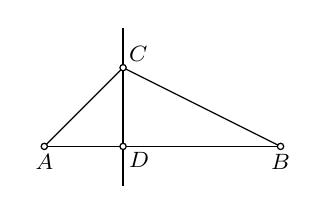
\begin{tikzpicture}
                    % \clip (0,0) rectangle (14.000000,10.000000);
                    {\footnotesize
                    
                    % Drawing segment A B
                    \draw [line width=0.016cm] (1.540000,1.500000) -- (2.460000,1.500000);%
                    \draw [line width=0.016cm] (2.540000,1.500000) -- (4.460000,1.500000);%
                    
                    % Drawing segment A C
                    \draw [line width=0.016cm] (1.528284,1.528284) -- (2.471716,2.471716);%
                    
                    % Drawing segment B C
                    \draw [line width=0.016cm] (4.464223,1.517889) -- (2.535777,2.482111);%
                    
                    % Drawing line s
                    \draw [line width=0.016cm] (2.500000,1.000000) -- (2.500000,1.460000);%
                    \draw [line width=0.016cm] (2.500000,1.540000) -- (2.500000,2.460000);%
                    \draw [line width=0.016cm] (2.500000,2.540000) -- (2.500000,3.000000);%
                    
                    % Marking point A by circle
                    \draw [line width=0.016cm] (1.500000,1.500000) circle (0.040000);%
                    \draw (1.500000,1.500000) node [anchor=north] { $A$ };%
                    
                    % Marking point B by circle
                    \draw [line width=0.016cm] (4.500000,1.500000) circle (0.040000);%
                    \draw (4.500000,1.500000) node [anchor=north] { $B$ };%
                    
                    % Marking point D by circle
                    \draw [line width=0.016cm] (2.500000,1.500000) circle (0.040000);%
                    \draw (2.470000,1.530000) node [anchor=north west] { $D$ };%
                    
                    % Marking point C by circle
                    \draw [line width=0.016cm] (2.500000,2.500000) circle (0.040000);%
                    \draw (2.470000,2.470000) node [anchor=south west] { $C$ };%
                    }
                    \end{tikzpicture}
                \\ Iščemo pravokotni trikotnik z $\delta=0$. Ker je v trikotniku vsota kotov manjša/enaka $\pi$, ima trikotnik vsaj dva ostra kota, tj. velikosti manj kot $\frac{\pi}{2}$. Naj bosta to kota $\angle A$ in $\angle B$. Naj bo $p$ pravokotnica skozi točko $C$ na $\overleftrightarrow{AB}$ in točka $D$ presečišče $p$ in $\overleftrightarrow{AB}$. Trdimo: \dashuline{$A\ast D\ast B$}. Če je $D$ izven $AB$, dobimo trikotnik z večjim notranjim kotom kot je nasprotni zunanji kot. Ker je $A\ast D\ast B$, sledi $\delta(\triangle ADC)=0$ (pravokotni trikotnik). 
                Iz pravokotnega trikotnika $\triangle ADC$ lahko konstruiramo pravokotnik: 
                \\ 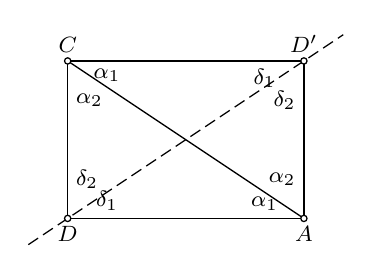
\begin{tikzpicture}
                    % \clip (0,0) rectangle (14.000000,10.000000);
                    {\footnotesize
                    
                    % Drawing segment A D
                    \draw [line width=0.016cm] (4.460000,1.500000) -- (1.540000,1.500000);%
                    
                    % Drawing segment D' A
                    \draw [line width=0.016cm] (4.500000,3.460000) -- (4.500000,1.540000);%
                    
                    % Drawing segment D' C
                    \draw [line width=0.016cm] (4.460000,3.500000) -- (1.540000,3.500000);%
                    
                    % Drawing segment D C
                    \draw [line width=0.016cm] (1.500000,1.540000) -- (1.500000,3.460000);%
                    
                    % Drawing segment C A
                    \draw [line width=0.016cm] (1.533282,3.477812) -- (4.466718,1.522188);%
                    
                    % Drawing line D D'
                    \draw [line width=0.016cm] (1.000000,1.166667) -- (1.124808,1.249872);%
                    \draw [line width=0.016cm] (1.187211,1.291474) -- (1.312019,1.374679);%
                    \draw [line width=0.016cm] (1.374423,1.416282) -- (1.466718,1.477812);%
                    \draw [line width=0.016cm] (1.561634,1.541089) -- (1.686441,1.624294);%
                    \draw [line width=0.016cm] (1.748845,1.665897) -- (1.873653,1.749102);%
                    \draw [line width=0.016cm] (1.936057,1.790704) -- (2.060864,1.873909);%
                    \draw [line width=0.016cm] (2.123268,1.915512) -- (2.248075,1.998717);%
                    \draw [line width=0.016cm] (2.310479,2.040319) -- (2.435287,2.123525);%
                    \draw [line width=0.016cm] (2.497691,2.165127) -- (2.622498,2.248332);%
                    \draw [line width=0.016cm] (2.684902,2.289935) -- (2.809709,2.373140);%
                    \draw [line width=0.016cm] (2.872113,2.414742) -- (2.996921,2.497947);%
                    \draw [line width=0.016cm] (3.059324,2.539550) -- (3.184132,2.622755);%
                    \draw [line width=0.016cm] (3.246536,2.664357) -- (3.371343,2.747562);%
                    \draw [line width=0.016cm] (3.433747,2.789165) -- (3.558555,2.872370);%
                    \draw [line width=0.016cm] (3.620958,2.913972) -- (3.745766,2.997177);%
                    \draw [line width=0.016cm] (3.808170,3.038780) -- (3.932977,3.121985);%
                    \draw [line width=0.016cm] (3.995381,3.163587) -- (4.120189,3.246792);%
                    \draw [line width=0.016cm] (4.182592,3.288395) -- (4.307400,3.371600);%
                    \draw [line width=0.016cm] (4.369804,3.413202) -- (4.466718,3.477812);%
                    \draw [line width=0.016cm] (4.557015,3.538010) -- (4.681823,3.621215);%
                    \draw [line width=0.016cm] (4.744226,3.662818) -- (4.869034,3.746023);%
                    \draw [line width=0.016cm] (4.931438,3.787625) -- (5.000000,3.833333);%
                    
                    % Marking point A by circle
                    \draw [line width=0.016cm] (4.500000,1.500000) circle (0.040000);%
                    \draw (4.500000,1.500000) node [anchor=north] { $A$ };%
                    
                    % Marking point D by circle
                    \draw [line width=0.016cm] (1.500000,1.500000) circle (0.040000);%
                    \draw (1.500000,1.500000) node [anchor=north] { $D$ };%
                    
                    % Marking point C by circle
                    \draw [line width=0.016cm] (1.500000,3.500000) circle (0.040000);%
                    \draw (1.500000,3.500000) node [anchor=south] { $C$ };%
                    
                    % Marking point D' by circle
                    \draw [line width=0.016cm] (4.500000,3.500000) circle (0.040000);%
                    \draw (4.500000,3.500000) node [anchor=south] { $D'$ };%
                    
                    % Marking point \alpha_1
                    \draw (4.000000,1.500000) node [anchor=south] { $\alpha_1$ };%
                    
                    % Marking point \alpha_2
                    \draw (4.500000,2.000000) node [anchor=east] { $\alpha_2$ };%
                    
                    % Marking point \alpha_1
                    \draw (2.000000,3.500000) node [anchor=north] { $\alpha_1$ };%
                    
                    % Marking point \alpha_2
                    \draw (1.500000,3.000000) node [anchor=west] { $\alpha_2$ };%
                    
                    % Marking point \delta_1
                    \draw (2.000000,1.500000) node [anchor=south] { $\delta_1$ };%
                    
                    % Marking point \delta_2
                    \draw (1.500000,2.000000) node [anchor=west] { $\delta_2$ };%
                    
                    % Marking point \delta_1
                    \draw (4.000000,3.500000) node [anchor=north] { $\delta_1$ };%
                    
                    % Marking point \delta_2
                    \draw (4.500000,3.000000) node [anchor=east] { $\delta_2$ };%
                    }
                    \end{tikzpicture}                    
                \\ $0=\delta(\triangle ADC)=\pi-(\alpha_1+\frac{\pi}{2}+\alpha_2)$ \ $\Rightarrow \alpha_1+\alpha_2 = \frac{\pi}{2}$. Torej so vsi koti pravi.
                \item Dovolj je dokazati, da imajo vsi pravokotni trikotniki $\delta=0$. Začnemo s pravokotnikom $\Box ABCD$. Iz tega lahko konstruiramo pravokotnik (pokažemo obstoj), ki ima stranici poljubno dolgi (skupaj zložimo več pravokotnikov). 
                \\ 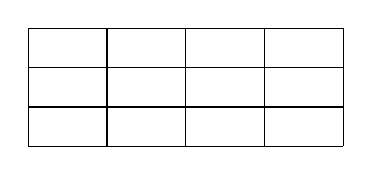
\begin{tikzpicture}
                    % \clip (0,0) rectangle (14.000000,10.000000);
                    {\footnotesize
                    
                    % Drawing segment A E
                    \draw [line width=0.016cm] (1.500000,1.500000) -- (5.500000,1.500000);%
                    
                    % Drawing segment A H
                    \draw [line width=0.016cm] (1.500000,1.500000) -- (1.500000,3.000000);%
                    
                    % Drawing segment F M
                    \draw [line width=0.016cm] (1.500000,2.000000) -- (5.500000,2.000000);%
                    
                    % Drawing segment G N
                    \draw [line width=0.016cm] (1.500000,2.500000) -- (5.500000,2.500000);%
                    
                    % Drawing segment B I
                    \draw [line width=0.016cm] (2.500000,1.500000) -- (2.500000,3.000000);%
                    
                    % Drawing segment C J
                    \draw [line width=0.016cm] (3.500000,1.500000) -- (3.500000,3.000000);%
                    
                    % Drawing segment D K
                    \draw [line width=0.016cm] (4.500000,1.500000) -- (4.500000,3.000000);%
                    
                    % Drawing segment E L
                    \draw [line width=0.016cm] (5.500000,1.500000) -- (5.500000,3.000000);%
                    
                    % Drawing segment H L
                    \draw [line width=0.016cm] (1.500000,3.000000) -- (5.500000,3.000000);%
                    }
                    \end{tikzpicture}                    
                \\ Za poljuben pravokotni trikotnik $\triangle EFG$ obstaja pravokotnik, ki ga vsebuje. 
                \\ 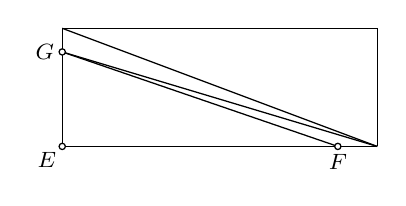
\begin{tikzpicture}
                    % \clip (0,0) rectangle (14.000000,10.000000);
                    {\footnotesize
                    
                    % Marking point G by circle
                    \draw [line width=0.016cm] (1.500000,2.700000) circle (0.040000);%
                    \draw (1.500000,2.700000) node [anchor=east] { $G$ };%
                    
                    % Marking point E by circle
                    \draw [line width=0.016cm] (1.500000,1.500000) circle (0.040000);%
                    \draw (1.530000,1.530000) node [anchor=north east] { $E$ };%
                    
                    % Marking point F by circle
                    \draw [line width=0.016cm] (5.000000,1.500000) circle (0.040000);%
                    \draw (5.000000,1.500000) node [anchor=north] { $F$ };%
                    
                    % Drawing segment E H
                    \draw [line width=0.016cm] (1.540000,1.500000) -- (4.960000,1.500000);%
                    \draw [line width=0.016cm] (5.040000,1.500000) -- (5.500000,1.500000);%
                    
                    % Drawing segment E I
                    \draw [line width=0.016cm] (1.500000,1.540000) -- (1.500000,2.660000);%
                    \draw [line width=0.016cm] (1.500000,2.740000) -- (1.500000,3.000000);%
                    
                    % Drawing segment H I
                    \draw [line width=0.016cm] (5.500000,1.500000) -- (1.500000,3.000000);%
                    
                    % Drawing segment H J
                    \draw [line width=0.016cm] (5.500000,1.500000) -- (5.500000,3.000000);%
                    
                    % Drawing segment I J
                    \draw [line width=0.016cm] (1.500000,3.000000) -- (5.500000,3.000000);%
                    
                    % Drawing segment G F
                    \draw [line width=0.016cm] (1.537838,2.687027) -- (4.962162,1.512973);%
                    
                    % Drawing segment H G
                    \draw [line width=0.016cm] (5.500000,1.500000) -- (1.538313,2.688506);%
                    }
                    \end{tikzpicture}                    
                \\ Če pravokotnik razdelimo z diagonalo, dobimo dva trikotnika z $\delta=0$: vsota kotov v pravokotniku je $2\pi$ in je enaka vsoti vseh vsot kotov v nastalih trikotnikih. Ker ima vsak trikotnik vsoto kotov manjšo/enako $\pi$, morata imeti oba trikotnika vsoto kotov enako $\pi$, torej $\delta=0$.
            \end{enumerate}
        \end{dokaz}

    \begin{posledica}
        Bodisi imajo vsi trikotniki $\delta=0$ (Evklidska geometrija) bodisi imajo vsi trikotniki $\delta>0$ (hiperbolična geometrija).
    \end{posledica}


\section{Aksiomi o vzporednicah}

    Te aksiome bomo obravnavali kot izjave v nevtralni geometriji.

    \begin{aksiom}[Hilbertov aksiom]
        Za poljubno premico $p$ in točko $A\notin p$ obstaja natanko ena vzporednica k premici $p$ skozi točko $A$.
    \end{aksiom}

        \begin{tikzpicture}
            % \clip (0,0) rectangle (14.000000,10.000000);
            {\footnotesize
            
            % Marking point A by circle
            \draw [line width=0.016cm] (5.000000,6.000000) circle (0.040000);%
            \draw (5.030000,5.970000) node [anchor=south east] { $A$ };%
            
            % Marking point p
            \draw (7.000000,4.500000) node [anchor=south east] { $p$ };%
            
            % Marking point q
            \draw (6.702703,6.283784) node [anchor=south east] { $q$ };%
            
            % Drawing line r
            \draw [line width=0.016cm] (1.000000,3.500000) -- (8.500000,4.750000);%
            
            % Drawing line s
            \draw [line width=0.016cm] (1.000000,5.333333) -- (4.960544,5.993424);%
            \draw [line width=0.016cm] (5.039456,6.006576) -- (8.500000,6.583333);%
            }
        \end{tikzpicture}

    \begin{opomba}
        Vemo, da v nevtralni geometriji obstaja vsaj ena vzporednica, zato bi v Hilbertovem aksiomu lahko zahtevali, da obstaja 'največ ena' vzporednica.
    \end{opomba}

    \begin{aksiom}[Evklidov aksiom]
        Če premica $t$ seka premici $p$ in $q$ tako, da je vsota notranjih kotov na enem bregu premice $t$ manjša od $\pi$, potem se premici $p$ in $q$ sekata na tem bregu premice $t$.
    \end{aksiom}

        \begin{tikzpicture}
            % \clip (0,0) rectangle (14.000000,10.000000);
            {\footnotesize
            
            % Drawing line T
            \draw [line width=0.016cm] (1.666667,1.000000) -- (2.666667,4.000000);%
            
            % Drawing line Q
            \draw [line width=0.016cm] (1.000000,3.500000) -- (6.245714,3.500000);%
            \draw [line width=0.016cm] (6.325714,3.500000) -- (7.000000,3.500000);%
            
            % Drawing line P
            \draw [line width=0.016cm] (1.000000,1.650000) -- (6.247960,3.486786);%
            \draw [line width=0.016cm] (6.323469,3.513214) -- (7.000000,3.750000);%
            
            % Marking point q
            \draw (4.000000,3.500000) node [anchor=south east] { $q$ };%
            
            % Marking point p
            \draw (4.000000,2.700000) node [anchor=south east] { $p$ };%
            
            % Marking point \alpha
            \draw (2.500000,3.500000) node [anchor=north west] { $\alpha$ };%
            
            % Marking point \beta
            \draw (2.000000,2.000000) node [anchor=south west] { $\beta$ };%
            
            % Marking point W by circle
            \draw [line width=0.016cm] (6.285714,3.500000) circle (0.040000);%
            
            % Marking point t
            \draw (2.262368,2.787103) node [anchor=south east] { $t$ };%
            }
        \end{tikzpicture}

    \begin{izrek}
        Hilbertov aksiom $\Leftrightarrow$ Evklidov aksiom.
    \end{izrek}

        \begin{dokaz}
            \\ ($\Rightarrow$):
            \\ 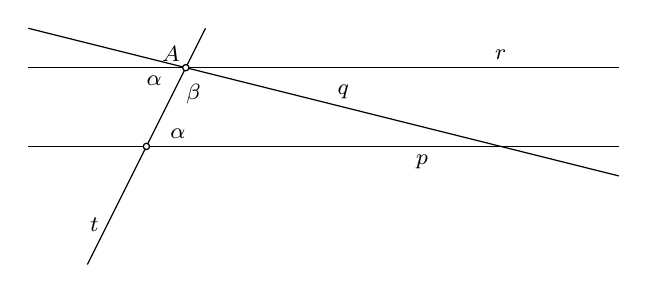
\begin{tikzpicture}
                % \clip (0,0) rectangle (14.000000,10.000000);
                {\footnotesize
                
                % Drawing line P
                \draw [line width=0.016cm] (1.000000,2.500000) -- (2.460000,2.500000);%
                \draw [line width=0.016cm] (2.540000,2.500000) -- (8.500000,2.500000);%
                
                % Drawing line R
                \draw [line width=0.016cm] (1.000000,3.500000) -- (2.960000,3.500000);%
                \draw [line width=0.016cm] (3.040000,3.500000) -- (8.500000,3.500000);%
                
                % Drawing line Q
                \draw [line width=0.016cm] (1.000000,4.000000) -- (2.961194,3.509701);%
                \draw [line width=0.016cm] (3.038806,3.490299) -- (8.500000,2.125000);%
                
                % Drawing line T
                \draw [line width=0.016cm] (1.750000,1.000000) -- (2.482111,2.464223);%
                \draw [line width=0.016cm] (2.517889,2.535777) -- (2.982111,3.464223);%
                \draw [line width=0.016cm] (3.017889,3.535777) -- (3.250000,4.000000);%
                
                % Marking point t
                \draw (2.000000,1.500000) node [anchor=east] { $t$ };%
                
                % Marking point r
                \draw (7.000000,3.500000) node [anchor=south] { $r$ };%
                
                % Marking point p
                \draw (6.000000,2.500000) node [anchor=north] { $p$ };%
                
                % Marking point q
                \draw (5.000000,3.000000) node [anchor=south] { $q$ };%
                
                % Marking point A by circle
                \draw [line width=0.016cm] (3.000000,3.500000) circle (0.040000);%
                \draw (3.030000,3.470000) node [anchor=south east] { $A$ };%
                
                % Marking point I by circle
                \draw [line width=0.016cm] (2.500000,2.500000) circle (0.040000);%
                
                % Marking point \alpha
                \draw (2.900000,2.500000) node [anchor=south] { $\alpha$ };%
                
                % Marking point \alpha
                \draw (2.600000,3.500000) node [anchor=north] { $\alpha$ };%
                
                % Marking point \beta
                \draw (3.100000,3.400000) node [anchor=north] { $\beta$ };%
                }
                \end{tikzpicture}
            \\ $\alpha+\beta<\pi$. Naj bo $A=t\cap q$ in $r$ premica skozi točko $A$ tako, da oklepata premici $p$ in $r$ s premico $t$ skladna izmenična notranja kota. Ker je $\alpha+\beta<\pi$, sledi: $r\neq q$. Potem je $r\parallel p$. Po Hilbertovem aksiomu sledi $q \nparallel p$, zato se $p$ in $q$ sekata in morata se sekati na isti  strani kot sta kota $\alpha$ in $\beta$ (zaradi vsote kotov v trikotniku oziroma izreka o prečnici).
            \\ ($\Leftarrow$):
            \\ 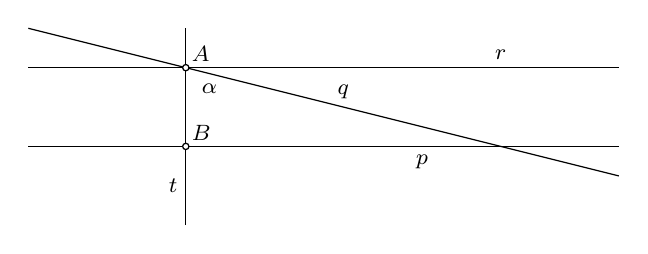
\begin{tikzpicture}
                % \clip (0,0) rectangle (14.000000,10.000000);
                {\footnotesize
                
                % Drawing line P
                \draw [line width=0.016cm] (1.000000,2.500000) -- (2.960000,2.500000);%
                \draw [line width=0.016cm] (3.040000,2.500000) -- (8.500000,2.500000);%
                
                % Drawing line R
                \draw [line width=0.016cm] (1.000000,3.500000) -- (2.960000,3.500000);%
                \draw [line width=0.016cm] (3.040000,3.500000) -- (8.500000,3.500000);%
                
                % Drawing line Q
                \draw [line width=0.016cm] (1.000000,4.000000) -- (2.961194,3.509701);%
                \draw [line width=0.016cm] (3.038806,3.490299) -- (8.500000,2.125000);%
                
                % Drawing line T
                \draw [line width=0.016cm] (3.000000,1.500000) -- (3.000000,2.460000);%
                \draw [line width=0.016cm] (3.000000,2.540000) -- (3.000000,3.460000);%
                \draw [line width=0.016cm] (3.000000,3.540000) -- (3.000000,4.000000);%
                
                % Marking point t
                \draw (3.000000,2.000000) node [anchor=east] { $t$ };%
                
                % Marking point r
                \draw (7.000000,3.500000) node [anchor=south] { $r$ };%
                
                % Marking point p
                \draw (6.000000,2.500000) node [anchor=north] { $p$ };%
                
                % Marking point q
                \draw (5.000000,3.000000) node [anchor=south] { $q$ };%
                
                % Marking point A by circle
                \draw [line width=0.016cm] (3.000000,3.500000) circle (0.040000);%
                \draw (2.970000,3.470000) node [anchor=south west] { $A$ };%
                
                % Marking point I by circle
                \draw [line width=0.016cm] (3.000000,2.500000) circle (0.040000);%
                \draw (2.970000,2.470000) node [anchor=south west] { $B$ };%
                
                % Marking point \alpha
                \draw (3.300000,3.400000) node [anchor=north] { $\alpha$ };%
                }
                \end{tikzpicture}                
            \\ Naj bo premica $t$ pravokotnica skozi točko $A$ na premico $p$ in $r$ pravokotnica na premico $t$ skozi točko $A$. Vemo: $r \parallel p$. Naj bo $q$ poljubna druga premica skozi točko $A$. Eden od poltrakov $q$ iz $A$ oklepa s poltrakom $\overrightarrow{AB}$ kot $\alpha<\frac{\pi}{2}$. Na tem bregu premice $t$ je vsota notranjih kotov, ki jih s premico $t$ oklepata premici $p$ in $q$ manjša od $\pi$. Po Evklidovem aksiomu sledi: premici $p$ in $q$ se sekata.
        \end{dokaz}

    \begin{izrek}
        Naj bodo $p, q, r, t$ premice. Potem so naslednje trditve ekvivalentne:
        \begin{enumerate}
            \item Hilbertov aksiom o vzporednicah
            \item Če je $p\parallel q$ in $q \parallel r$, potem je $p\parallel r$.
            \item Če je $p\parallel q$ in $p$ seka $t$, potem $q$ seka $t$.
            \item (I.29) Če je $p\parallel q$ in $t$ seka $p$ in $q$, potem sta izmenična notranja kota skladna.
        \end{enumerate}
    \end{izrek}

        \begin{dokaz}
            \\ ($1 \Rightarrow 4$): 
            \\ 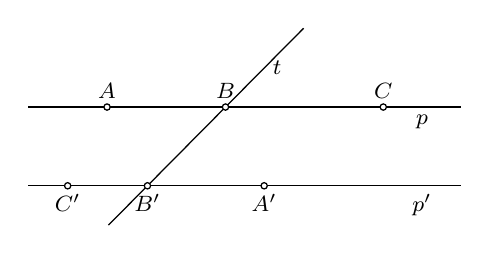
\begin{tikzpicture}
                % \clip (0,0) rectangle (14.000000,10.000000);
                {\footnotesize
                
                % Drawing line P
                \draw [line width=0.016cm] (1.000000,2.500000) -- (1.960000,2.500000);%
                \draw [line width=0.016cm] (2.040000,2.500000) -- (3.464323,2.500000);%
                \draw [line width=0.016cm] (3.544323,2.500000) -- (5.468055,2.500000);%
                \draw [line width=0.016cm] (5.548055,2.500000) -- (6.500000,2.500000);%
                
                % Drawing line C' p'
                \draw [line width=0.016cm] (1.000000,1.500000) -- (1.460000,1.500000);%
                \draw [line width=0.016cm] (1.540000,1.500000) -- (2.472970,1.500000);%
                \draw [line width=0.016cm] (2.552970,1.500000) -- (3.955493,1.500000);%
                \draw [line width=0.016cm] (4.035493,1.500000) -- (6.500000,1.500000);%
                
                % Drawing line T
                \draw [line width=0.016cm] (2.017294,1.000000) -- (2.484809,1.471593);%
                \draw [line width=0.016cm] (2.541132,1.528407) -- (3.476162,2.471593);%
                \draw [line width=0.016cm] (3.532485,2.528407) -- (4.495677,3.500000);%
                
                % Marking point A by circle
                \draw [line width=0.016cm] (2.000000,2.500000) circle (0.040000);%
                \draw (2.000000,2.500000) node [anchor=south] { $A$ };%
                
                % Marking point B by circle
                \draw [line width=0.016cm] (3.504323,2.500000) circle (0.040000);%
                \draw (3.504323,2.500000) node [anchor=south] { $B$ };%
                
                % Marking point C by circle
                \draw [line width=0.016cm] (5.508055,2.500000) circle (0.040000);%
                \draw (5.508055,2.500000) node [anchor=south] { $C$ };%
                
                % Marking point p
                \draw (6.000000,2.500000) node [anchor=north] { $p$ };%
                
                % Marking point p'
                \draw (6.000000,1.500000) node [anchor=north] { $p'$ };%
                
                % Marking point t
                \draw (4.000000,3.000000) node [anchor=west] { $t$ };%
                
                % Marking point C' by circle
                \draw [line width=0.016cm] (1.500000,1.500000) circle (0.040000);%
                \draw (1.500000,1.500000) node [anchor=north] { $C'$ };%
                
                % Marking point B' by circle
                \draw [line width=0.016cm] (2.512970,1.500000) circle (0.040000);%
                \draw (2.512970,1.500000) node [anchor=north] { $B'$ };%
                
                % Marking point A' by circle
                \draw [line width=0.016cm] (3.995493,1.500000) circle (0.040000);%
                \draw (3.995493,1.500000) node [anchor=north] { $A'$ };%
                }
                \end{tikzpicture}                
            \\ Privzemimo najprej, da v nevtralni ravnini velja Hilbertov aksiom in naj bosta $p$ in $p'$ vzporednici ter $t$ prečnica, ki ju seka v točkah $B$ in $B'$. Izberimo točki $A, C \in p$, da je $A\ast B\ast C$ in točki $A', C' \in p'$, da je $A'\ast B'\ast C'$. Nadalje privzemimo, da sta $A$ in $A'$ na nasprotnih bregovih premice $t$. Pokazati moramo, da potem velja $\angle C'B'B \cong\angle CBB'$ in $\angle A'B'B\cong\angle ABB'$. Pa denimo, da je $\angle C'B'B <\angle CBB'$. Potem bi bilo tudi $\angle C'B'B + \angle ABB' < \angle CBB' + \angle ABB' =\pi$, kjer smo s $\pi$ označili vsoto dveh pravih kotov. Po Evklidovem aksiomu o vzporednosti bi od tod sledilo, da se premici $p$ in $p'$ sekata na bregu, ki vsebuje točki $A$ in $C'$. To pa nas pripelje v protislovje s predpostavko, da sta $p$ in $p'$ vzporedni. Podobno bi nas do protislovja pripeljala predpostavka, da je $\angle C'B'B > \angle CBB'$, zato mora po zakonu o trihotomiji veljati $\angle C'B'B\cong\angle CBB'$. Ker sta sokota skladnih kotov spet skladna, mora veljati tudi $\angle A'B'B\cong\angle ABB'$. 
            \\ ($4 \Rightarrow 1$): 
            \\ 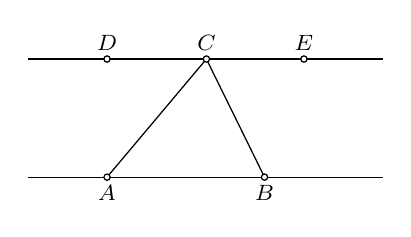
\begin{tikzpicture}
                % \clip (0,0) rectangle (14.000000,10.000000);
                {\footnotesize
                
                % Drawing line A B
                \draw [line width=0.016cm] (1.000000,1.500000) -- (1.960000,1.500000);%
                \draw [line width=0.016cm] (2.040000,1.500000) -- (3.960000,1.500000);%
                \draw [line width=0.016cm] (4.040000,1.500000) -- (5.500000,1.500000);%
                
                % Drawing line D E
                \draw [line width=0.016cm] (1.000000,3.000000) -- (1.960000,3.000000);%
                \draw [line width=0.016cm] (2.040000,3.000000) -- (3.222017,3.000000);%
                \draw [line width=0.016cm] (3.302017,3.000000) -- (4.460000,3.000000);%
                \draw [line width=0.016cm] (4.540000,3.000000) -- (5.500000,3.000000);%
                
                % Drawing segment A C
                \draw [line width=0.016cm] (2.025752,1.530608) -- (3.236265,2.969392);%
                
                % Drawing segment C B
                \draw [line width=0.016cm] (3.279675,2.964109) -- (3.982342,1.535891);%
                
                % Marking point D by circle
                \draw [line width=0.016cm] (2.000000,3.000000) circle (0.040000);%
                \draw (2.000000,3.000000) node [anchor=south] { $D$ };%
                
                % Marking point E by circle
                \draw [line width=0.016cm] (4.500000,3.000000) circle (0.040000);%
                \draw (4.500000,3.000000) node [anchor=south] { $E$ };%
                
                % Marking point C by circle
                \draw [line width=0.016cm] (3.262017,3.000000) circle (0.040000);%
                \draw (3.262017,3.000000) node [anchor=south] { $C$ };%
                
                % Marking point B by circle
                \draw [line width=0.016cm] (4.000000,1.500000) circle (0.040000);%
                \draw (4.000000,1.500000) node [anchor=north] { $B$ };%
                
                % Marking point A by circle
                \draw [line width=0.016cm] (2.000000,1.500000) circle (0.040000);%
                \draw (2.000000,1.500000) node [anchor=north] { $A$ };%
                }
                \end{tikzpicture}                
            \\ Sedaj bomo privzeli, da v nevtralni ravnini velja aksiom o izmeničnih kotih. Namesto Evklidovega aksioma o vzporednosti pa bomo od tod izpeljali ekvivalenten aksiom, da je vsota notranjih kotov v trikotniku enaka $\pi$. Izberimo poljuben trikotnik $\triangle ABC$ in izberimo točki $D$ in $E$, da je $\overleftrightarrow{DE}$ vzporedna $\overleftrightarrow{AB}$ in da je $D \ast C \ast E$. Po aksiomu o izmeničnih kotih potem velja $\angle BAC \cong \angle DCA$ in $\angle ABC \cong \angle ECB$. Od tod sledi $\angle BAC +\angle ABC +\angle ACB \cong \angle DCA + \angle ECB + \angle ACB = \pi$.
            \\ ($1 \Rightarrow 2$): 
            \\ 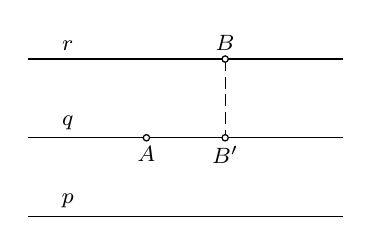
\begin{tikzpicture}
                % \clip (0,0) rectangle (14.000000,10.000000);
                {\footnotesize
                
                % Drawing line p p'
                \draw [line width=0.016cm] (1.000000,1.500000) -- (5.000000,1.500000);%
                
                % Drawing line q q'
                \draw [line width=0.016cm] (1.000000,2.500000) -- (2.460000,2.500000);%
                \draw [line width=0.016cm] (2.540000,2.500000) -- (3.460000,2.500000);%
                \draw [line width=0.016cm] (3.540000,2.500000) -- (5.000000,2.500000);%
                
                % Drawing line r r'
                \draw [line width=0.016cm] (1.000000,3.500000) -- (3.460000,3.500000);%
                \draw [line width=0.016cm] (3.540000,3.500000) -- (5.000000,3.500000);%
                
                % Drawing segment B B'
                \draw [line width=0.016cm] (3.500000,3.460000) -- (3.500000,3.350000);%
                \draw [line width=0.016cm] (3.500000,3.275000) -- (3.500000,3.125000);%
                \draw [line width=0.016cm] (3.500000,3.050000) -- (3.500000,2.900000);%
                \draw [line width=0.016cm] (3.500000,2.825000) -- (3.500000,2.675000);%
                \draw [line width=0.016cm] (3.500000,2.600000) -- (3.500000,2.540000);%
                
                % Marking point A by circle
                \draw [line width=0.016cm] (2.500000,2.500000) circle (0.040000);%
                \draw (2.500000,2.500000) node [anchor=north] { $A$ };%
                
                % Marking point B' by circle
                \draw [line width=0.016cm] (3.500000,2.500000) circle (0.040000);%
                \draw (3.500000,2.500000) node [anchor=north] { $B'$ };%
                
                % Marking point B by circle
                \draw [line width=0.016cm] (3.500000,3.500000) circle (0.040000);%
                \draw (3.500000,3.500000) node [anchor=south] { $B$ };%
                
                % Marking point p
                \draw (1.500000,1.500000) node [anchor=south] { $p$ };%
                
                % Marking point q
                \draw (1.500000,2.500000) node [anchor=south] { $q$ };%
                
                % Marking point r
                \draw (1.500000,3.500000) node [anchor=south] { $r$ };%
                }
                \end{tikzpicture}                
            \\ Naj bo $p$ neka premica in točki $A$ in $B$ takšni, da velja $A,B\notin p$ in $A\neq B$. Po Hilbertu obstaja taka premica $q$ skozi $A$ vzporedna premici $p$ in obstaja taka premica $r$ skozi $B$ vzporedna premici $q$. Naj bo $B'$ pravokotna projekcija točke $B$ na premico $q$. Obstaja enolično določena premica $q'$ skozi $B'$ vzporedna $p$. Ker $B'$ pripada tudi premici $q$, potem velja $q'=q$. Torej točki $A$ in $B'$ ležita tako na $q$ in $q'$. Potem je $r$ vzporedna $p$.
            \\ ($2 \Rightarrow 1$): 
            \\ 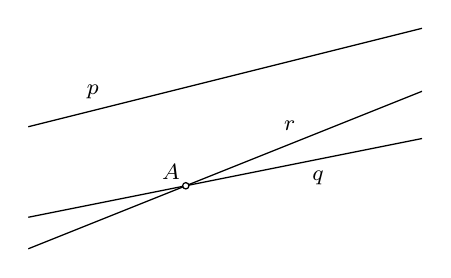
\begin{tikzpicture}
                % \clip (0,0) rectangle (14.000000,10.000000);
                {\footnotesize
                
                % Drawing line p X
                \draw [line width=0.016cm] (6.000000,4.500000) -- (1.000000,3.250000);%
                
                % Drawing line A q
                \draw [line width=0.016cm] (1.000000,2.100000) -- (2.960777,2.492155);%
                \draw [line width=0.016cm] (3.039223,2.507845) -- (6.000000,3.100000);%
                
                % Drawing line A r
                \draw [line width=0.016cm] (1.000000,1.700000) -- (2.962861,2.485144);%
                \draw [line width=0.016cm] (3.037139,2.514856) -- (6.000000,3.700000);%
                
                % Marking point A by circle
                \draw [line width=0.016cm] (3.000000,2.500000) circle (0.040000);%
                \draw (3.030000,2.470000) node [anchor=south east] { $A$ };%
                
                % Marking point p
                \draw (2.000000,3.500000) node [anchor=south east] { $p$ };%
                
                % Marking point q
                \draw (4.500000,2.800000) node [anchor=north west] { $q$ };%
                
                % Marking point r
                \draw (4.500000,3.100000) node [anchor=south east] { $r$ };%
                }
                \end{tikzpicture}                
            \\ Naj bo $p$ premica in $A$ točka, ki ne pripada $p$. Recimo, da sta premici $q$ in $r$ različni vzporednici k premici $p$ skozi točko $A$. Potem se sekata v točki $A$: $\{A\}=r\cap q\neq\emptyset$. Velja pa tudi tranzitivnost $p\parallel q \wedge p\parallel r \Rightarrow r\parallel q$, in zato $q\parallel r$. Iz tega pa sledi $q=r$.
            \\ ($1 \Rightarrow 3$): 
            \\ 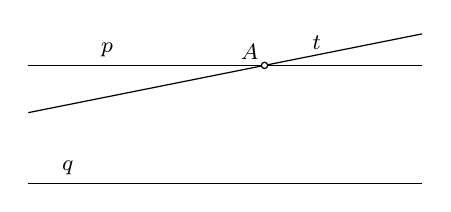
\begin{tikzpicture}
                % \clip (0,0) rectangle (14.000000,10.000000);
                {\footnotesize
                
                % Drawing line p X
                \draw [line width=0.016cm] (1.000000,1.500000) -- (6.000000,1.500000);%
                
                % Drawing line A q
                \draw [line width=0.016cm] (1.000000,3.000000) -- (3.960000,3.000000);%
                \draw [line width=0.016cm] (4.040000,3.000000) -- (6.000000,3.000000);%
                
                % Drawing line A t
                \draw [line width=0.016cm] (1.000000,2.400000) -- (3.960777,2.992155);%
                \draw [line width=0.016cm] (4.039223,3.007845) -- (6.000000,3.400000);%
                
                % Marking point A by circle
                \draw [line width=0.016cm] (4.000000,3.000000) circle (0.040000);%
                \draw (4.030000,2.970000) node [anchor=south east] { $A$ };%
                
                % Marking point p
                \draw (1.500000,1.500000) node [anchor=south] { $q$ };%
                
                % Marking point q
                \draw (2.000000,3.000000) node [anchor=south] { $p$ };%
                
                % Marking point t
                \draw (4.500000,3.100000) node [anchor=south west] { $t$ };%
                }
                \end{tikzpicture}                
            \\ Naj bosta $p$ in $q$ vzporedni premici in naj bo $t$ taka premica, ki seka premico $p$ v neki točki $A$. Recimo, da premica $t$ ne seka premice $q$. Potem je $t\parallel q$, zaradi tranzitivnosti pa velja tudi $t\parallel p$. To nas pripelje v protislovje ($t\cap p=A$). Torej $t$ seka tako premico $p$ kot njeno vzporednico $q$.
            \\ ($3 \Rightarrow 1$): 
            \\ 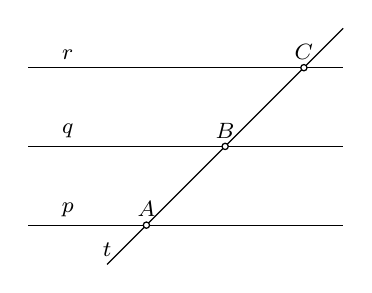
\begin{tikzpicture}
                % \clip (0,0) rectangle (14.000000,10.000000);
                {\footnotesize
                
                % Drawing line T
                \draw [line width=0.016cm] (2.000000,1.000000) -- (2.471716,1.471716);%
                \draw [line width=0.016cm] (2.528284,1.528284) -- (3.471716,2.471716);%
                \draw [line width=0.016cm] (3.528284,2.528284) -- (4.471716,3.471716);%
                \draw [line width=0.016cm] (4.528284,3.528284) -- (5.000000,4.000000);%
                
                % Drawing line p p'
                \draw [line width=0.016cm] (1.000000,1.500000) -- (2.460000,1.500000);%
                \draw [line width=0.016cm] (2.540000,1.500000) -- (5.000000,1.500000);%
                
                % Drawing line q q'
                \draw [line width=0.016cm] (1.000000,2.500000) -- (3.460000,2.500000);%
                \draw [line width=0.016cm] (3.540000,2.500000) -- (5.000000,2.500000);%
                
                % Drawing line r r'
                \draw [line width=0.016cm] (1.000000,3.500000) -- (4.460000,3.500000);%
                \draw [line width=0.016cm] (4.540000,3.500000) -- (5.000000,3.500000);%
                
                % Marking point A by circle
                \draw [line width=0.016cm] (2.500000,1.500000) circle (0.040000);%
                \draw (2.500000,1.500000) node [anchor=south] { $A$ };%
                
                % Marking point C by circle
                \draw [line width=0.016cm] (4.500000,3.500000) circle (0.040000);%
                \draw (4.500000,3.500000) node [anchor=south] { $C$ };%
                
                % Marking point B by circle
                \draw [line width=0.016cm] (3.500000,2.500000) circle (0.040000);%
                \draw (3.500000,2.500000) node [anchor=south] { $B$ };%
                
                % Marking point p
                \draw (1.500000,1.500000) node [anchor=south] { $p$ };%
                
                % Marking point q
                \draw (1.500000,2.500000) node [anchor=south] { $q$ };%
                
                % Marking point r
                \draw (1.500000,3.500000) node [anchor=south] { $r$ };%
                
                % Marking point t
                \draw (2.000000,1.000000) node [anchor=south] { $t$ };%
                }
                \end{tikzpicture}                
            \\ Naj bo $p$ premica in $q$ njena vzporednica skozi točko $B$, $B\notin p$. Naj bo $r$ vzporednica k premici $q$. Premica $t$ naj poteka skozi točko $B$. Ker sta $p\parallel q$, vemo, da $t$ seka tudi $p$, to točko označimo z $A$. Ker pa sta $r\parallel q$, potem $t$ seka tudi premico $r$, to točko označimo s $C$. Recimo, da je $p\cap r\neq \emptyset$, potem je tudi $p\cap q\neq\emptyset$, kar nas privede v protislovje ($p\parallel q$). Torej je $r$ vzporedna $p$.
        \end{dokaz}

    \begin{trditev}[I.32]
        Hilbertov aksiom $\Rightarrow$ defekt poljubnega trikotnika je $0$ ($\delta(\triangle ABC)=0$) -- vsota kotov v trikotniku je $\pi$.
    \end{trditev}

        \begin{dokaz}
            \\ 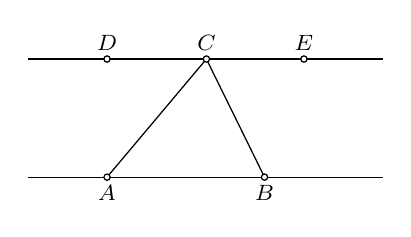
\begin{tikzpicture}
                % \clip (0,0) rectangle (14.000000,10.000000);
                {\footnotesize
                
                % Drawing line A B
                \draw [line width=0.016cm] (1.000000,1.500000) -- (1.960000,1.500000);%
                \draw [line width=0.016cm] (2.040000,1.500000) -- (3.960000,1.500000);%
                \draw [line width=0.016cm] (4.040000,1.500000) -- (5.500000,1.500000);%
                
                % Drawing line D E
                \draw [line width=0.016cm] (1.000000,3.000000) -- (1.960000,3.000000);%
                \draw [line width=0.016cm] (2.040000,3.000000) -- (3.222017,3.000000);%
                \draw [line width=0.016cm] (3.302017,3.000000) -- (4.460000,3.000000);%
                \draw [line width=0.016cm] (4.540000,3.000000) -- (5.500000,3.000000);%
                
                % Drawing segment A C
                \draw [line width=0.016cm] (2.025752,1.530608) -- (3.236265,2.969392);%
                
                % Drawing segment C B
                \draw [line width=0.016cm] (3.279675,2.964109) -- (3.982342,1.535891);%
                
                % Marking point D by circle
                \draw [line width=0.016cm] (2.000000,3.000000) circle (0.040000);%
                \draw (2.000000,3.000000) node [anchor=south] { $D$ };%
                
                % Marking point E by circle
                \draw [line width=0.016cm] (4.500000,3.000000) circle (0.040000);%
                \draw (4.500000,3.000000) node [anchor=south] { $E$ };%
                
                % Marking point C by circle
                \draw [line width=0.016cm] (3.262017,3.000000) circle (0.040000);%
                \draw (3.262017,3.000000) node [anchor=south] { $C$ };%
                
                % Marking point B by circle
                \draw [line width=0.016cm] (4.000000,1.500000) circle (0.040000);%
                \draw (4.000000,1.500000) node [anchor=north] { $B$ };%
                
                % Marking point A by circle
                \draw [line width=0.016cm] (2.000000,1.500000) circle (0.040000);%
                \draw (2.000000,1.500000) node [anchor=north] { $A$ };%
                }
                \end{tikzpicture}                
            \\ Naj bo $\triangle ABC$ trikotnik in premica $q$ skozi $C$ naj bo vzporedna premici $\overleftrightarrow{AB}$ (po Hilbertovem aksiomu). Na premici $q$ izberemo točki $D$ in $E$ tako, da velja $D\ast C\ast E$ in $D$ leži na nasprotnem bregu premice $\overleftrightarrow{AC}$ kot $B$. Po izreku o izmeničnih kotih velja: $\angle BAC\cong\angle ACD$ in $\angle ABC\cong\angle BCE$. Ker so točke $D, E, C$ kolinearne, je $\angle DCE =\pi$ in $\angle DCE=\angle ACD + \angle ACB + \angle BCE$, torej je $\angle BAC + \angle ACB + \angle ABC = \pi$. Torej je defekt enak: $\delta(\triangle ABC)= \pi-(\angle BAC + \angle ABC + \angle ACB)=\pi - \pi = 0$.
        \end{dokaz}

    \begin{aksiom}[hiperbolični aksiom]
        Obstaja premica $p$ in točka $A\notin p$, da skozi točko $A$ potekata vsaj dve vzporednici k premici $p$.
    \end{aksiom}

    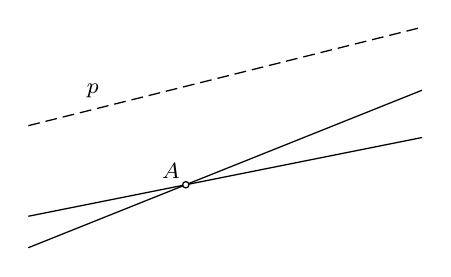
\begin{tikzpicture}
        % \clip (0,0) rectangle (14.000000,10.000000);
        {\footnotesize
        
        % Drawing line p X
        \draw [line width=0.016cm] (1.000000,3.250000) -- (1.145521,3.286380);%
        \draw [line width=0.016cm] (1.218282,3.304571) -- (1.363803,3.340951);%
        \draw [line width=0.016cm] (1.436564,3.359141) -- (1.582086,3.395521);%
        \draw [line width=0.016cm] (1.654846,3.413712) -- (1.800368,3.450092);%
        \draw [line width=0.016cm] (1.873128,3.468282) -- (2.018650,3.504662);%
        \draw [line width=0.016cm] (2.091410,3.522853) -- (2.236932,3.559233);%
        \draw [line width=0.016cm] (2.309692,3.577423) -- (2.455214,3.613803);%
        \draw [line width=0.016cm] (2.527974,3.631994) -- (2.673496,3.668374);%
        \draw [line width=0.016cm] (2.746257,3.686564) -- (2.891778,3.722944);%
        \draw [line width=0.016cm] (2.964539,3.741135) -- (3.110060,3.777515);%
        \draw [line width=0.016cm] (3.182821,3.795705) -- (3.328342,3.832086);%
        \draw [line width=0.016cm] (3.401103,3.850276) -- (3.546624,3.886656);%
        \draw [line width=0.016cm] (3.619385,3.904846) -- (3.764906,3.941227);%
        \draw [line width=0.016cm] (3.837667,3.959417) -- (3.983188,3.995797);%
        \draw [line width=0.016cm] (4.055949,4.013987) -- (4.201470,4.050368);%
        \draw [line width=0.016cm] (4.274231,4.068558) -- (4.419752,4.104938);%
        \draw [line width=0.016cm] (4.492513,4.123128) -- (4.638034,4.159509);%
        \draw [line width=0.016cm] (4.710795,4.177699) -- (4.856316,4.214079);%
        \draw [line width=0.016cm] (4.929077,4.232269) -- (5.074599,4.268650);%
        \draw [line width=0.016cm] (5.147359,4.286840) -- (5.292881,4.323220);%
        \draw [line width=0.016cm] (5.365641,4.341410) -- (5.511163,4.377791);%
        \draw [line width=0.016cm] (5.583923,4.395981) -- (5.729445,4.432361);%
        \draw [line width=0.016cm] (5.802205,4.450551) -- (5.947727,4.486932);%
        
        % Drawing line A Y
        \draw [line width=0.016cm] (1.000000,2.100000) -- (2.960777,2.492155);%
        \draw [line width=0.016cm] (3.039223,2.507845) -- (6.000000,3.100000);%
        
        % Drawing line A Z
        \draw [line width=0.016cm] (1.000000,1.700000) -- (2.962861,2.485144);%
        \draw [line width=0.016cm] (3.037139,2.514856) -- (6.000000,3.700000);%
        
        % Marking point A by circle
        \draw [line width=0.016cm] (3.000000,2.500000) circle (0.040000);%
        \draw (3.030000,2.470000) node [anchor=south east] { $A$ };%
        
        % Marking point p
        \draw (2.000000,3.500000) node [anchor=south east] { $p$ };%
        }
    \end{tikzpicture}        

    \begin{opomba}
        To je negacija Hilbertovega aksioma.
    \end{opomba}

    \begin{trditev}
        Hiperbolični aksiom $\Rightarrow$ obstaja trikotnik s pozitivnim defektom.
    \end{trditev}

        \begin{dokaz}
            \\ 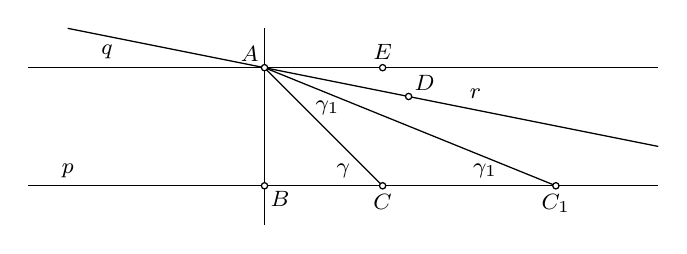
\begin{tikzpicture}
                % \clip (0,0) rectangle (14.000000,10.000000);
                {\footnotesize
                
                % Drawing line p X
                \draw [line width=0.016cm] (1.000000,1.500000) -- (3.960000,1.500000);%
                \draw [line width=0.016cm] (4.040000,1.500000) -- (5.460000,1.500000);%
                \draw [line width=0.016cm] (5.540000,1.500000) -- (7.660000,1.500000);%
                \draw [line width=0.016cm] (7.740000,1.500000) -- (9.000000,1.500000);%
                
                % Drawing line b
                \draw [line width=0.016cm] (4.000000,1.000000) -- (4.000000,1.460000);%
                \draw [line width=0.016cm] (4.000000,1.540000) -- (4.000000,2.960000);%
                \draw [line width=0.016cm] (4.000000,3.040000) -- (4.000000,3.500000);%
                
                % Drawing line A q
                \draw [line width=0.016cm] (1.000000,3.000000) -- (3.960000,3.000000);%
                \draw [line width=0.016cm] (4.040000,3.000000) -- (5.460000,3.000000);%
                \draw [line width=0.016cm] (5.540000,3.000000) -- (9.000000,3.000000);%
                
                % Drawing line A r
                \draw [line width=0.016cm] (1.500000,3.500000) -- (3.960777,3.007845);%
                \draw [line width=0.016cm] (4.039223,2.992155) -- (5.790819,2.641836);%
                \draw [line width=0.016cm] (5.869266,2.626147) -- (9.000000,2.000000);%
                
                % Drawing segment A C
                \draw [line width=0.016cm] (4.028284,2.971716) -- (5.471716,1.528284);%
                
                % Drawing segment A C_1
                \draw [line width=0.016cm] (4.037070,2.984972) -- (7.662930,1.515028);%
                
                % Marking point A by circle
                \draw [line width=0.016cm] (4.000000,3.000000) circle (0.040000);%
                \draw (4.030000,2.970000) node [anchor=south east] { $A$ };%
                
                % Marking point p
                \draw (1.500000,1.500000) node [anchor=south] { $p$ };%
                
                % Marking point q
                \draw (2.000000,3.000000) node [anchor=south] { $q$ };%
                
                % Marking point r
                \draw (6.500000,2.500000) node [anchor=south west] { $r$ };%
                
                % Marking point D by circle
                \draw [line width=0.016cm] (5.830042,2.633992) circle (0.040000);%
                \draw (5.800042,2.603992) node [anchor=south west] { $D$ };%
                
                % Marking point B by circle
                \draw [line width=0.016cm] (4.000000,1.500000) circle (0.040000);%
                \draw (3.970000,1.530000) node [anchor=north west] { $B$ };%
                
                % Marking point C by circle
                \draw [line width=0.016cm] (5.500000,1.500000) circle (0.040000);%
                \draw (5.500000,1.500000) node [anchor=north] { $C$ };%
                
                % Marking point C_1 by circle
                \draw [line width=0.016cm] (7.700000,1.500000) circle (0.040000);%
                \draw (7.700000,1.500000) node [anchor=north] { $C_1$ };%
                
                % Marking point E by circle
                \draw [line width=0.016cm] (5.500000,3.000000) circle (0.040000);%
                \draw (5.500000,3.000000) node [anchor=south] { $E$ };%

                % Marking point \gamma
                \draw (5.000000,1.500000) node [anchor=south] { $\gamma$ };%
                
                % Marking point \gamma_1
                \draw (6.800000,1.500000) node [anchor=south] { $\gamma_1$ };%
                
                % Marking point \gamma_1
                \draw (4.800000,2.300000) node [anchor=south] { $\gamma_1$ };%
                }
                \end{tikzpicture}                
            \\ Naj bo premica $q$ standardna vzporednica k premici $p$. Po hiperboličnem aksiomu obstaja še ena vzporedna premica $r$ skozi točko $A$ k premici $p$. Izberimo točko $C$ na premici $p$ na tistem bregu premice $t$, kjer poltrak $\overrightarrow{AD}$ na $r$ iz $A$ leži med premicama $p$ in $q$. Potem je $\angle BAC<\angle BAD$, saj mora biti $\overrightarrow{AC}$ znotraj kota $\angle BAD$ (sicer bi $\overrightarrow{AD}$ po izreku o prečnici sekala $p$). Če lahko izberemo točko $C$ tako, da bo $|\angle ACB|<|\angle DAE|$, potem bo $\delta(\triangle ABC)>0$ (vsota kotov pri $A$ in $C$ manjša od $\frac{\pi}{2}$).
            Naj bo $C_1\in p$, $B\ast C\ast C_1$ in $CC_1\cong AC$. Potem je $2\gamma_1<\gamma$ (vsota dveh kotov v trikotniku je manjša od nasprotnega zunanjega kota). Sledi: $\gamma_1<\frac{\gamma}{2}$. Po nekaj korakih dosežemo, da je $|\angle ACB|<|\angle DAE|$.
        \end{dokaz}

    \begin{posledica}
        Hilbertov aksiom $\Leftrightarrow$ $\delta(\triangle)=0$
        \\ Hiperbolični aksiom $\Leftrightarrow$ $\delta(\triangle)>0$ $\Leftrightarrow$ pravokotniki ne obstajajo.
    \end{posledica}

    \begin{trditev}[univerzalni hiperbolični aksiom]
        Če velja hiperbolični aksiom, potem za vsako premico $p$ in vsako točko $A\notin p$, potekata skozi točko $A$ vsaj dve vzporednici k premici $p$.
    \end{trditev}

        \begin{dokaz}
            \\ 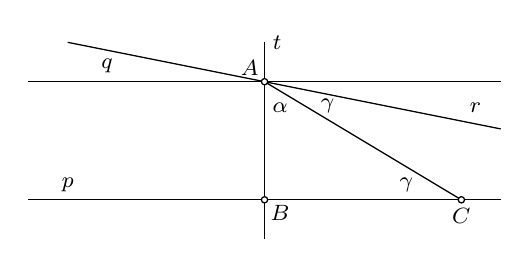
\begin{tikzpicture}
                % \clip (0,0) rectangle (14.000000,10.000000);
                {\footnotesize
                
                % Drawing line p X
                \draw [line width=0.016cm] (1.000000,1.500000) -- (3.960000,1.500000);%
                \draw [line width=0.016cm] (4.040000,1.500000) -- (6.460000,1.500000);%
                \draw [line width=0.016cm] (6.540000,1.500000) -- (7.000000,1.500000);%
                
                % Drawing line b
                \draw [line width=0.016cm] (4.000000,1.000000) -- (4.000000,1.460000);%
                \draw [line width=0.016cm] (4.000000,1.540000) -- (4.000000,2.960000);%
                \draw [line width=0.016cm] (4.000000,3.040000) -- (4.000000,3.500000);%
                
                % Drawing line A q
                \draw [line width=0.016cm] (1.000000,3.000000) -- (3.960000,3.000000);%
                \draw [line width=0.016cm] (4.040000,3.000000) -- (7.000000,3.000000);%
                
                % Drawing line A r
                \draw [line width=0.016cm] (1.500000,3.500000) -- (3.960777,3.007845);%
                \draw [line width=0.016cm] (4.039223,2.992155) -- (7.000000,2.400000);%
                
                % Drawing segment A C
                \draw [line width=0.016cm] (4.034300,2.979420) -- (6.465700,1.520580);%
                
                % Marking point A by circle
                \draw [line width=0.016cm] (4.000000,3.000000) circle (0.040000);%
                \draw (4.030000,2.970000) node [anchor=south east] { $A$ };%
                
                % Marking point p
                \draw (1.500000,1.500000) node [anchor=south] { $p$ };%
                
                % Marking point q
                \draw (2.000000,3.000000) node [anchor=south] { $q$ };%
                
                % Marking point r
                \draw (6.500000,2.500000) node [anchor=south west] { $r$ };%
                
                % Marking point t
                \draw (4.000000,3.500000) node [anchor=west] { $t$ };%
                
                % Marking point B by circle
                \draw [line width=0.016cm] (4.000000,1.500000) circle (0.040000);%
                \draw (3.970000,1.530000) node [anchor=north west] { $B$ };%
                
                % Marking point C by circle
                \draw [line width=0.016cm] (6.500000,1.500000) circle (0.040000);%
                \draw (6.500000,1.500000) node [anchor=north] { $C$ };%
                
                % Marking point \gamma
                \draw (5.800000,1.500000) node [anchor=south] { $\gamma$ };%
                
                % Marking point \alpha
                \draw (4.200000,2.500000) node [anchor=south] { $\alpha$ };%
                
                % Marking point \gamma
                \draw (4.800000,2.500000) node [anchor=south] { $\gamma$ };%
                }
                \end{tikzpicture}                
            \\ Naj bo premica $q$ standardna vzporednica k premici $p$ skozi točko $A$ in točka $C\in p$ različna od $B=p\cap t$. $\delta(\triangle ABC)>0 \Rightarrow \alpha+\gamma<\frac{\pi}{2}$. Po I.27 sta si premici $p$ in $r$ vzporedni: s premico $\overleftrightarrow{AC}$ oklepata skladna izmenična notranja kota ($\gamma$).
        \end{dokaz}

    \begin{trditev}[KKK]
        Hiperbolični aksiom $\Rightarrow$ skladnostni kriterij KKK za trikotnik: če imata trikotnika skladne istoležne kote, sta skladna.
    \end{trditev}

        \begin{dokaz}
            \\ 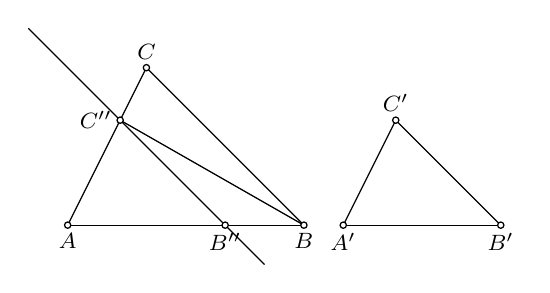
\begin{tikzpicture}
                % \clip (0,0) rectangle (14.000000,10.000000);
                {\footnotesize
                
                % Drawing segment A C
                \draw [line width=0.016cm] (1.517889,1.535777) -- (2.148778,2.797556);%
                \draw [line width=0.016cm] (2.184555,2.869110) -- (2.482111,3.464223);%
                
                % Drawing segment A B
                \draw [line width=0.016cm] (1.540000,1.500000) -- (3.460000,1.500000);%
                \draw [line width=0.016cm] (3.540000,1.500000) -- (4.460000,1.500000);%
                
                % Drawing segment C B
                \draw [line width=0.016cm] (2.528284,3.471716) -- (4.471716,1.528284);%
                
                % Drawing segment A' B'
                \draw [line width=0.016cm] (5.040000,1.500000) -- (6.960000,1.500000);%
                
                % Drawing segment B' C'
                \draw [line width=0.016cm] (6.971716,1.528284) -- (5.694951,2.805049);%
                
                % Drawing segment A' C'
                \draw [line width=0.016cm] (5.017889,1.535777) -- (5.648778,2.797556);%
                
                % Drawing segment B C''
                \draw [line width=0.016cm] (4.465270,1.519846) -- (2.201396,2.813488);%
                
                % Drawing line a''
                \draw [line width=0.016cm] (4.000000,1.000000) -- (3.528284,1.471716);%
                \draw [line width=0.016cm] (3.471716,1.528284) -- (2.194951,2.805049);%
                \draw [line width=0.016cm] (2.138382,2.861618) -- (1.000000,4.000000);%
                
                % Marking point A by circle
                \draw [line width=0.016cm] (1.500000,1.500000) circle (0.040000);%
                \draw (1.500000,1.500000) node [anchor=north] { $A$ };%
                
                % Marking point B by circle
                \draw [line width=0.016cm] (4.500000,1.500000) circle (0.040000);%
                \draw (4.500000,1.500000) node [anchor=north] { $B$ };%
                
                % Marking point A' by circle
                \draw [line width=0.016cm] (5.000000,1.500000) circle (0.040000);%
                \draw (5.000000,1.500000) node [anchor=north] { $A'$ };%
                
                % Marking point B' by circle
                \draw [line width=0.016cm] (7.000000,1.500000) circle (0.040000);%
                \draw (7.000000,1.500000) node [anchor=north] { $B'$ };%
                
                % Marking point C by circle
                \draw [line width=0.016cm] (2.500000,3.500000) circle (0.040000);%
                \draw (2.500000,3.500000) node [anchor=south] { $C$ };%
                
                % Marking point C' by circle
                \draw [line width=0.016cm] (5.666667,2.833333) circle (0.040000);%
                \draw (5.666667,2.833333) node [anchor=south] { $C'$ };%
                
                % Marking point B'' by circle
                \draw [line width=0.016cm] (3.500000,1.500000) circle (0.040000);%
                \draw (3.500000,1.500000) node [anchor=north] { $B''$ };%
                
                % Marking point C'' by circle
                \draw [line width=0.016cm] (2.166667,2.833333) circle (0.040000);%
                \draw (2.166667,2.833333) node [anchor=east] { $C''$ };%
                }
                \end{tikzpicture}                
            \\ Za trikotnika $\triangle ABC$ in $\triangle A'B'C'$ velja: $\angle A\cong \angle A';~\angle B\cong \angle B';~\angle C\cong \angle C'$.
            Če je $AB\cong A'B'$, skladnost trikotnikov sledi po kriteriju KSK.
            Denimo, da je $A'B'<AB$. Potem obstaja točka $B''$ taka, da je: $A\ast B''\ast B$ in $AB''\cong A'B'$. Naj bo $p$ premica skozi $B''$, ki s premico $\overleftrightarrow{AB}$ okepa kot skladen $\angle B'$. Po Paschevem izreku premica $p$ seka $AC$ ali $BC$, ampak ker je $BC\parallel p$ po I.27 (skladna izmenična notranja kota), sledi, da premica $p$ seka $AC$ v točki $C''$. Po KSK ($\angle A\cong\angle A';~AB''\cong A'B';~\angle B''\cong \angle B'$) sledi: $\triangle AB''C''\cong \triangle A'B'C'$. Zato velja: $\delta(\triangle AB''C'')=\delta(\triangle ABC)=\delta(\triangle AB''C'')+\delta(\triangle BB''C'')+\delta(\triangle BCC'')$. Od tod sledi: $\delta(\triangle BB''C'')=0=\delta(\triangle BCC'')$, kar je v protislovju s tem, da za vse trikotnike velja $\delta>0$. Torej velja: $\triangle ABC\cong\triangle A'B'C'$. 
        \end{dokaz}

    \begin{opomba}
        ~
        \begin{itemize}
            \item (Neskladni) podobni trikotniki obstajajo le v evklidski geometriji, ne pa tudi v hiperbolični geometriji.
            \item Ker imamo naravno enoto za merjenje kotov v nevtralni geometriji, od tod sledi, da v hiperbolični geometriji obstaja naravna enota za dolžino.
        \end{itemize}
    \end{opomba}

    \subsection{Zgodovina aksioma o vzporednicah}

        Že Evklid je imel pomisleke glede formulacije -- iskal je najbolj nazorno/preverljivo verzijo aksiom E.5. Prvič je ta aksiom uporabil v  I.29.

        Skoraj 2000 let so se matematiki trudili dokazati E.5 iz ostalih aksiomov  ali pa ga vsaj zamenjati s čim bolj nazornim.

        Prvi poskusi že v antiki (Ptolomej, Proklus), potem arabski/perzijski matematiki, do pomembnih zahodnih matematikov (Qallis, Saccheri, Lambert -- vsi so dokazovali E.5).

        Alternativno definicijo so postavili mnogi, npr. Clairaut je E.5 nadomestil s '\textit{pravokotniki obstajajo}', ki je bolj nazorna., a kot druge zamenjave logično ekvivalentna.

        Leta 1763 je G. S. Klügel spisal doktorat, v katerem je pokazal napake/implicitne privzetke v 28 dokazih E.5.

        Zgodba se konča okoli leta 1830:
        \begin{itemize}
            \item C. F. Gauss (1777--1855)
            \item F. Bolyai (1775--1856)
            \item J. Bolyai (1802--1860)
            \item N. L. Lobačevski (1792--1856)
        \end{itemize}

        Lobačevski objavi svoje rezultate o hiperbolični geometriji v Rusiji leta 1829, kjer je deležen hudih napadov, naj umakne svoje 'napačne' trditve. (Lobačevski je svoj prevod v nemščino dobil šele leta 1840.)

        F. Bolyai je objavil več 'dokazov' aksioma E.5, tudi še po tem, ko je njegov sin, J. Bolyai, leta 1831 v njegovi/očetovi knjigi o geometriji objavil svojo verzijo hiperbolične geometrije.

        Do Gaussove smrti leta 1855 hiperbolična geometrija ni bila splošno sprejeta. Po njegovi smrti, ko so bili objavljeni njegovi zapiski, o tem, in pisma, so tudi ostali to sprejeli.
        Po tem je geometrija doživela pravi razcvet, posebej z deli B.  Riemanna, ki je tvorec diferencialne geometrije, in je bil Gaussov učenec.
